\documentclass[12pt,a4paper,twoside]{report}
\usepackage[utf8]{inputenc}
\usepackage[english]{babel}
\usepackage{setspace}
\usepackage{amssymb,amsmath,amsfonts}
\usepackage{graphicx}
\usepackage{upquote} % quotes in verbatim environments
\usepackage{fixme}
\usepackage{microtype}
\usepackage[tmargin=3cm, lmargin=3cm, rmargin=3cm, bmargin=3cm, marginparsep=0.3cm, marginparwidth=2.4cm]{geometry}
\usepackage{hyperref}
\usepackage{import}
\usepackage{emptypage}
\PassOptionsToPackage{usenames,dvipsnames}{color} % color is loaded by hyperref
\hypersetup{unicode=true,
            colorlinks=true,
            linkcolor=black,
            citecolor=black,
            urlcolor=blue,
            breaklinks=true}
\urlstyle{same}  % don't use monospace font for urls
\usepackage{parskip}
\setlength{\emergencystretch}{3em}

\usepackage{algorithm}
\usepackage[end]{algpseudocode}
\let\Algorithm\algorithm
\renewcommand\algorithm[1][]{\Algorithm[#1]\setstretch{1.25}}

\usepackage[plain]{fancyref}
% Change references from capital/normal letters
\newcommand{\ffref}{\Fref}
% Algorithm and subsection references
\newcommand*{\fancyrefalglabelprefix}{alg}
\newcommand*{\fancyrefsubseclabelprefix}{subsec}
\frefformat{plain}{\fancyrefalglabelprefix}{%
algorithm\fancyrefdefaultspacing#1%
}
\Frefformat{plain}{\fancyrefalglabelprefix}{%
Algorithm\fancyrefdefaultspacing#1%
}
\frefformat{plain}{\fancyrefsubseclabelprefix}{%
subsection\fancyrefdefaultspacing#1%
}
\Frefformat{plain}{\fancyrefsubseclabelprefix}{%
Subsection\fancyrefdefaultspacing#1%
}
\frefformat{vario}{\fancyrefalglabelprefix}{%
algorithm\fancyrefdefaultspacing#1 on page~#2%
}
\Frefformat{vario}{\fancyrefalglabelprefix}{%
Algorithm\fancyrefdefaultspacing#1 on page~#2%
}
\frefformat{vario}{\fancyrefsubseclabelprefix}{%
subsection\fancyrefdefaultspacing#1 on page~#2%
}
\Frefformat{vario}{\fancyrefsubseclabelprefix}{%
Subsection\fancyrefdefaultspacing#1 on page~#2%
}

\usepackage{algpseudocode}
\algblockdefx[RepeatComment]{RepeatComment}{EndRepeatComment}
    [1][]{\textbf{repeat} #1}
    {\textbf{end repeat}}
\algblockdefx[RepeatUntilComment]{RepeatUntilComment}{EndRepeatUntilComment}
    [1][]{\textbf{repeat} #1}
    [1][]{\textbf{until} #1}

\usepackage{fancyhdr}
\setlength{\headheight}{15pt}
\fancyfoot{}
\fancyhead{}
\fancyhead[LE,RO]{\thepage}
\fancyhead[RE]{\nouppercase{\leftmark}}
\fancyhead[LO]{\nouppercase{\rightmark}}

%% Bibtex
\usepackage{csquotes}
%\usepackage[nottoc,numbib]{tocbibind}
\usepackage[numbib]{tocbibind}
\usepackage[style=authoryear,bibencoding=ascii,backend=bibtex,natbib]{biblatex}
\bibliographystyle{unsrt}
\addbibresource{report.bib}

%% Inkscape pdf_tex pictures
\usepackage{calc}
\def\svgscale{1}
\newcommand{\inkscapefig}[2]{
\begin{figure}[hbtp]
\begin{center}
  \subimport{img/}{#1.pdf_tex}
\end{center}
\caption{#2\label{fig:#1}}
\end{figure}
}

\usepackage[final]{pdfpages}

\usepackage{mfirstuc} % capitalisewords

%\newcommand{\newconceptspec}[2]{\emph{#1}\marginpar{\footnotesize\textsc{#2}}}
\newcommand{\newconceptspec}[2]{\emph{#1}}
\newcommand{\newconcept}[1]{\newconceptspec{#1}{\capitalisewords{#1}}}
\newcommand{\centeredtitle}[1]{ \phantomsection
  \addcontentsline{toc}{chapter}{#1} \begin{center} {\Huge
  \textbf{#1}} \end{center}\bigskip}
\newcommand{\argmin}{\operatornamewithlimits{arg\,min}}
\newcommand{\argmax}{\operatornamewithlimits{arg\,max}}

\subimport{Content/}{Acronyms.tex}


\begin{document}
\pagenumbering{roman}
\pagestyle{empty}
%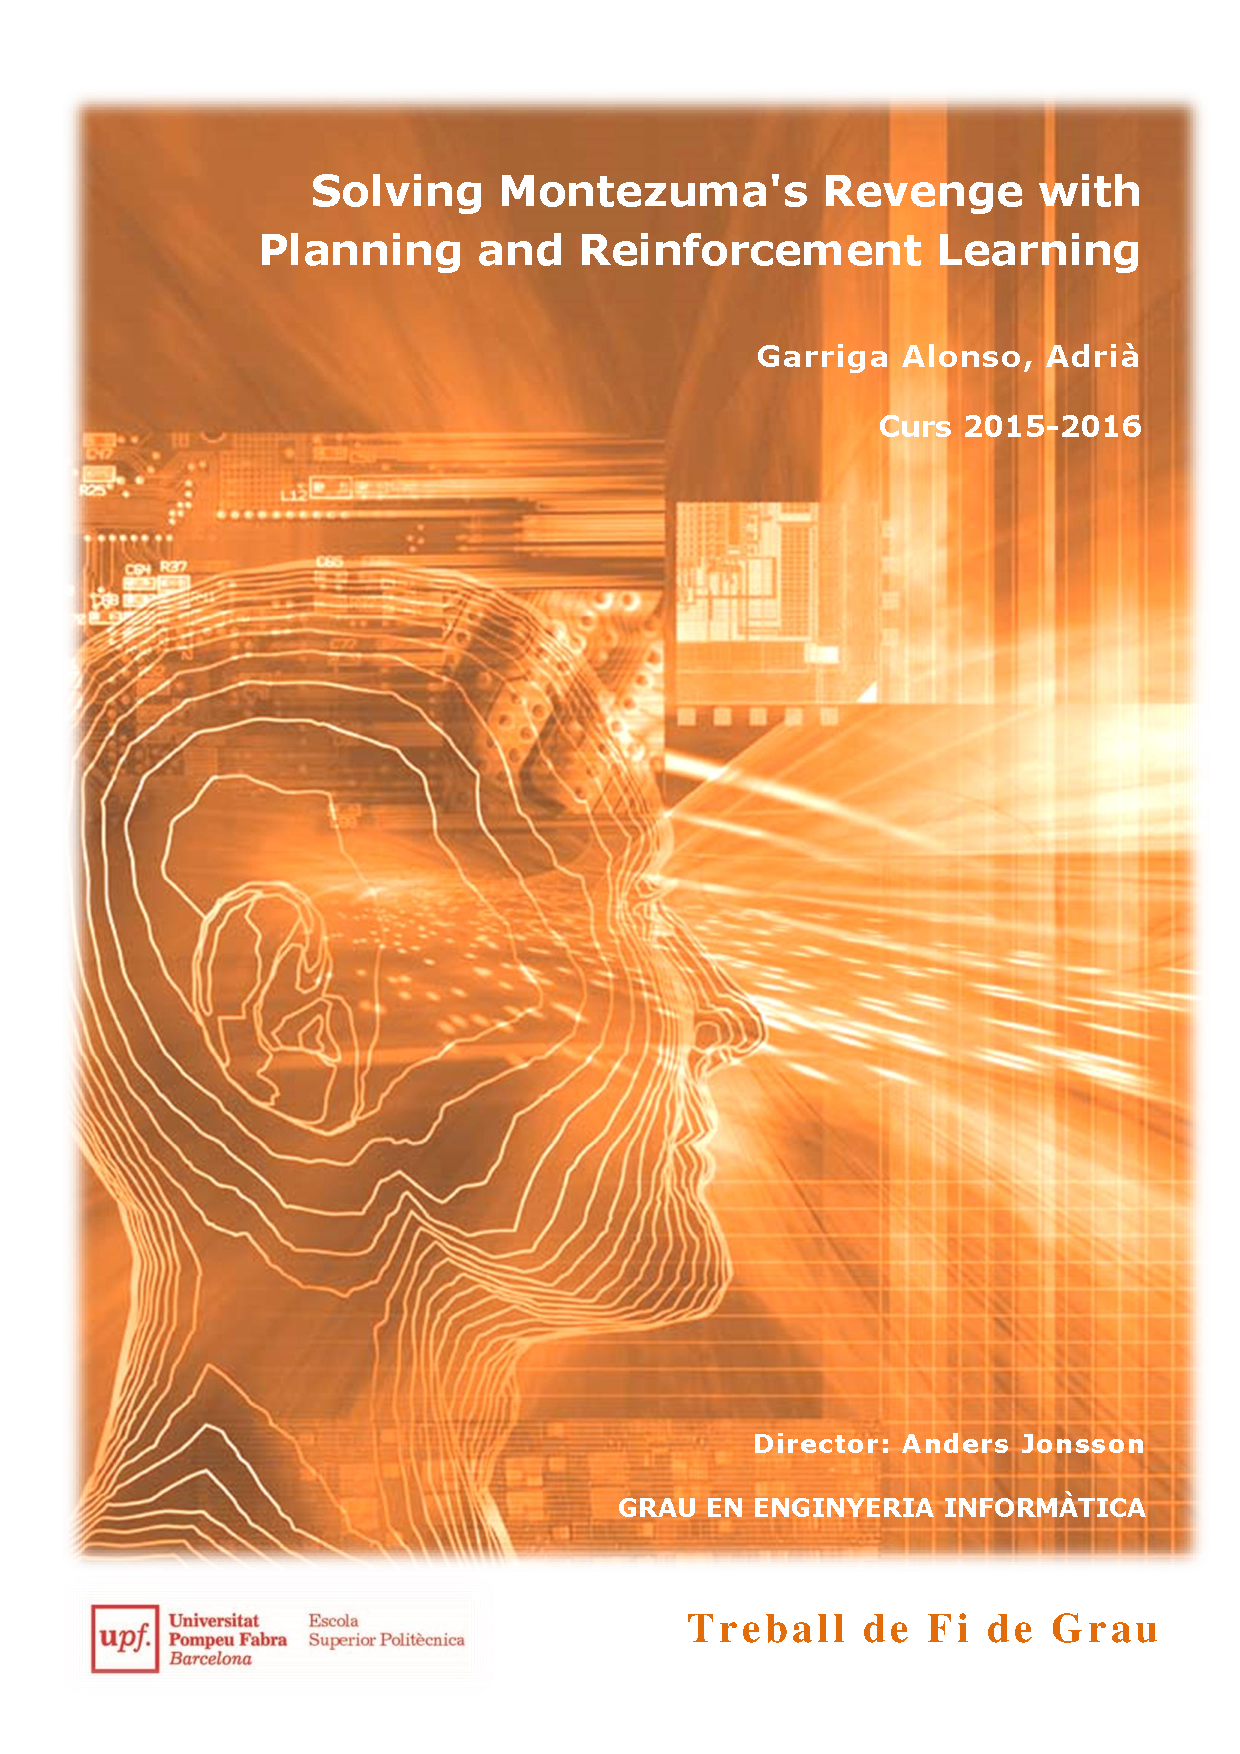
\includepdf[pages={1}]{Content/cover.pdf}
%\cleardoublepage
{\hypersetup{urlcolor=black}

\def\title{Solving Montezuma's Revenge with planning and reinforcement learning}
\def\subject{Planning \& Reinforcement Learning}
\def\keywords{Artificial Intelligence, Reinforcement Learning, Planning,
  Hierarchical Reinforcement Learning, Sparse, Intrinsic Motivation}
%\def\date{June 17, 2016}
\def\date{\today}

\def\authorName{Adrià Garriga Alonso}
\def\authorEmail{adria.garriga01@estudiant.upf.edu}

\def\supervisorName{Anders Jonsson}
\def\supervisorEmail{anders.jonsson@upf.edu}

\def\departmentName{Department of Information and Communication Technologies}
\def\departmentWeb{http://www.upf.edu/dtic/en/}

\def\degree{Bachelor in Computer Science}
\def\univlogo{img/logo_upf.jpg}


\def\author{\texorpdfstring
  {\href{mailto:\authorEmail}{\authorName}}
  {\authorName}
}
\def\supervisor{\texorpdfstring
  {\href{mailto:\supervisorEmail}{\supervisorName}}
  {\supervisorName}
}
\def\department{\texorpdfstring
  {\href{\departmentWeb}{\departmentName}}
  {\departmentName}
}

\hypersetup{pdftitle={\title}}
\hypersetup{pdfsubject=\subject}
\hypersetup{pdfauthor=\author}
\hypersetup{pdfkeywords=\keywords}
\begin{titlepage}
  \setcounter{page}{3}
  \let\footnotesize\small
  \let\footnoterule\relax
  \let \footnote \thanks
  \setcounter{footnote}{0}
  \null\vfil
  \vskip 60pt
  \begin{center}
    \setlength{\parskip}{0pt}
    %{\large\textbf{\UNIVNAME}\par}
    %\vfill
    {\huge \bf \title \par}
    \bigskip
    \bigskip
    \bigskip
    \bigskip
    \bigskip
    %{\large by \par}
    \smallskip
    {\Large \author \par}
    \bigskip
    {\Large Supervised by \supervisor}
    \vfill
    {\Large \date \par}
%    \bigskip
%    {Edited \today}
    \vfill
    {\large \degree \par}
    \bigskip
    %{\large in the \par}
    %{\large \facname \par}
    {\large \department \par}
    \vfill
    \bigskip
    \bigskip
    \includegraphics[width=200px,height=100px, keepaspectratio]{\univlogo}
  \end{center}
%  \par
%  \@thanks
%  \vfil\null
\end{titlepage}
%\setcounter{footnote}{0}%
%\global\let\thanks\relax
%\global\let\maketitle\relax
%\global\let\thanks\@empty
%\global\let\author\@empty
%\global\let\date\@empty
%\global\let\title\@empty
%\global\let\title\relax
%\global\let\author\relax
%\global\let\date\relax
%\global\let\and\relax
}


\onehalfspacing

\cleardoublepage
\centeredtitle{Acknowledgements}

I wish to offer my thanks:

To my supervisor Anders Jonsson, for the guidance offered in navigating the
literature and in carrying out this project. I also want to thank him for
getting me interested into the fascinating field of \acs{RL}.

To my good friend and upperclassman Daniel Furelos, for being an academic role
model, and for the offered advice.

To Miquel Ramírez, for sharing the source code from his paper on Iterated Width,
along with Geffner and Lipovetzky.

To my parents and sister for the moral support, and the support of a noisy,
electricity-hungry computer that is continuously learning and planning.

\cleardoublepage
\centeredtitle{Abstract}

State-of-the-art methods for deep reinforcement learning have demonstrated the ability to learn complex game strategies.
However, they perform poorly in environments with sparse rewards or with the facility to die.
In both cases the algorithms are not able to learn from low probability rewards.
One of the algorithms that present this problem is \acf{A3C} (\cite{mnih2016A3C}).

For this project it has been developed an algorithm called \acf{MA3C} which uses transfer learning and hierarchial learning
to take advantage of subgoals.
The algorithm has been tested in three different environments, including Montezuma's Revenge, that presents both difficulties.
The experiments demonstrate that \ac{MA3C} explores better and learns more quickly just by using a few domain knowledge.

The proposed method is very flexible and generalizes to any environment where multiple subgoals can be defined.
Future research could be focused in the modification of this algorithm to automatically discover subgoals,
avoiding the usage of domain knowledge.

\cleardoublepage
%\lhead{Contents}
\pagestyle{fancy}
\tableofcontents

%\cleardoublepage
%\lhead{List of Figures}
%\listoffigures

%\cleardoublepage
%%\lhead{List of Tables}
%\listoftables

\cleardoublepage
\printacronyms[include-classes=abbrev,name=Abbreviations,heading=chapter*]
\phantomsection
\addcontentsline{toc}{chapter}{Abbreviations}

\cleardoublepage
\pagestyle{fancy}
\pagenumbering{arabic}
\chapter{Motivation}
Nature has the ability of evolving in all kinds of adverse environments.
One of the consequences of this continuous evolving is us, human beings,
the maximum expression of adaptive living being.
By using our intelligence we improve year by year the chances of survival
to this chaotic world.
This kind of intelligence is composed by several cognitive abilities: learning,
forming concepts, understanding, applying logic and reasoning.

Since creation of \acf{AI} investigators from all around
the world have tried to grant machines some of this skills.
One way of letting machines exhibit intelligence is by modeling how the human brain works.

The brain is composed by billions of neurons that interact with each other to create intelligence.
This system is named \acf{ANN} and scientists have learned lots of things about how it works,
but not everything.
Mathematicians used this knowledge to develop an artificial version of this network called
\acf{ANN}, which models neural networks based on mathematical functions.

But, why it is important for us to have intelligent machines?.
Because by teaching computers to do some tasks they will help us reducing the amount of work.
We can create intelligent tools to do our work better or to make our lives easier.

In the last years an area of \ac{AI} called \acf{RL} has become really popular.
In this field, algorithms learn how to solve any kind of tasks that has a numeric reward attached.
There are plenty of algorithms capables of learning abstractions of the problem to reuse its knowledge in similar ones.
Most of them are based on making decisions one after the other and looking how this choices change the environment.

The goal of this thesis is to extend a specific \ac{RL} algorithm based on \acp{ANN} to help machines solve complex tasks.

%%% Local Variables: 
%%% mode: latex
%%% TeX-master: "../report"
%%% End: 

\cleardoublepage
\chapter{Background}

\section{\aclp{RL}}
Reinforcement learning is an area of \acf{ML} that models a problem focusing on maximizing a numerical reward. To achieve this, the agent obtains a representation of the situation of the problem, named \newconcept{state}; then selects an \newconcept{action}; interacts with the environment, by applying that action; and finally it may obtain some \newconcept{reward}. After all this process the situation of the problem changes and the agent finds itself a new state. Repeating this steps several times, the agent should explore the different states of the problem and learn how to map situations to actions with the purpose of maximizing the reward.

The learning process is usually organized in \newconcept{episodes}. Each episode is composed by an initial state $s_0$ , the first one that the environment generates; intermediate states $s_t$ ; and may have several final states, which establish the end of an episode. The agent's goal is to maximize the total amount of reward it receives in a complete episode. When an episode ends the the environment resets and starts again from $s_0$ or some other initial state that belongs to the set of initial states. In some cases the agent interacts infinitely without reaching any terminal state, we call this \newconcept{continual tasks}.

One of the challenging aspects of reinforcement learning is the tradeoff between \newconcept{exploration} and \newconcept{exploitation}. In the kind of environments this thesis is focused on, the actions applied affect not only immediate rewards but also future ones. This implies that taking actions with high immediate reward is not always the best choice, there might be some series of actions with which it obtains higher rewards in the future. In reinforcement learning, the agent should exploit immediate rewards in order to obtain feedback of how is it performing. Nevertheless, it may also explore different actions that do not have as high immediate reward in order to find higher future rewards.

\subsection{The environment}
We will describe this as in the textbook \citetitle{sutton1998introduction} from \citet[Section~3.1]{sutton1998introduction}.

The \newconcept{environment} is the main source of information about the problem that we want to model with which the \newconcept{agent} is able to interact. This interactions and information about the problem must be stated in a specific way.

The state is the peace of information, from the environment, that our agent uses to make decisions. Interactions are transferred in the form of actions that the environment makes available for the agent. The information given about the problem must change based on the actions applied.

The agent and environment interact with each other in a sequence of discrete time steps, $t=0,1,2,\dots$ At each time step, $t$, the agent receives some state $s_t \in S$ and on that basis selects an action $a_t \in \methcal{A}( s_t )$. One time step later, the agent receives a numerical reward, $r_{t+1} \in \Re$, and finds itself a new state, $s_{t+1}$. The state transition and reward must depend on the sequence of past actions and states, if not the agent will not be able to figure out what to do for obtaining the highest rewards. The methodology in which the agent interacts step by step with the environment is named \acf{SDP}.

\inkscapefig{agent-environment}{Diagram of interaction between agent and
environment \citep[Section~3.1]{sutton1998introduction}}

This is an abstract and very flexible framework that fits in a large variety of problems. The different components of this interface can be arbitrarily defined to model different kinds of actions, time steps, states and environments. But it restricts rewards to the real domain. For example, the state can be any kind of information about the environment, from just an image of some maze to complex market statistics. This fact is important to us because the algorithm proposed in this thesis uses domain knowledge to define a state representation of the environment composed by images and additional information.

\subsection{\aclp{MDP}\label{subsec:MDP}}

A \acf{MDP} is a restricted case of \acp{SDP} (\cite[Section~3.5]{sutton1998introduction}). In \acp{MDP}, the state $s_{t+1}$ generated by applying action $a_t$ in state $s_t$ only depends on this two factors, unlike in \acp{SDP} that may depend on any previous states, rewards or actions. This fact is named the \newconcept{Markov property} and is formally described as:

\begin{equation}
    P \lbrace s_{t+1} = s, r_{t+1} = r | s_t,a_t,r_t,s_{t-1},a_{t-1}, \dots, r_1, s_0, a_0 \rbrace =
    P \lbrace s_{t+1} = s, r_{t+1} = r | s_t,a_t \rbrace
\end{equation}
As stated, the probability distribution over states and rewards only depends on the immediate previous state and action, not the full history. Bear in mind that the state $s_t$ may contain some representation of previous states, actions and rewards but not the full history. This abstract could be as simple as the number of actions taken.
All concepts presented in this thesis assumes that the environment can be defined as an MDP.
The problem can be expressed as a tuple $\langle\mathcal{S}, \mathcal{A}_s,
\mathcal{P}_a(s,s'), \mathcal{R}_a(s,s'), \gamma \rangle$ where:
\begin{itemize}
    \item $\mathcal{S}$ is the state space.
    \item $\mathcal{A}_s$ is the set of actions available in state $s$.
    \item $\mathcal{P}_a$ is the transition probability function
    $\mathcal{P}_a : \mathcal{S} \times \mathcal{S} \rightarrow [0,1]$
    for action $a \in \mathcal{A}_s$ . To clarify, $\mathcal{P}_a(s,s')$
    is the probability that taking action $a$ in state $s \in S$ will lead
    to state $s' ∈ S$.
    \item $\mathcal{R}_a$ is the reward function
    $\mathcal{R}_a : \mathcal{S} \times \mathcal{S} \rightarrow \Re$ for action
    $a \in \mathcal{A}_s$. To clarify, $\mathcal{R}_a(s,s')$ is the expected
    reward for transiting from state $s \in \mathcal{S}$ to state $s' \in \mathcal{S}$
    by taking action $a$.
    \item $\gamma \in [0,1]$ is the discount factor of future rewards used to calculate returns ( \ffref{subsec:returns} )
\end{itemize}

$\mathcal{S}$ and $\mathcal{A}_s$ may be infinite sets which implies that $\mathcal{P}_a(s,s')$ and $\mathcal{R}_a(s,s')$ may
also be infinite. If this happens the MDP is named \newconconcept{infinite MDP}.

\subsection{Returns\label{subsec:returns}}

We have defined the goal of the agent, that is to maximize the total reward obtained in an episode. We also said that the agent must learn to reach that goal, but we have not defined yet how the agent should select the actions to achieve it. The expected return $R$ must be defined in a way that encourages the agent to learn, so $R$ is some specific function of the reward sequence. The simplest way of computing it is just adding all the future rewards.
\begin{equation}
    R_t=r_{t+1}+r_{t+2}+r_{t+3}+...+r_T
\end{equation}
Where $r_T$ is the reward obtained in some terminal state. In continual tasks the
time step $T = \inf$ so the return, which is what we are trying to maximize, will also be infinite. To avoid this problem we must introduce
the \newconcept{discounted return}, which adds in a discount factor $\gamma$. This factor modifies the previous formulation in the following way:
\begin{equation}
    R_t = r_{t+1} + \gamma r_{t+2} + \gamma^2 r_{t+3} + \dots = \sum_{k=0}^\infty\gamma^k r_{t+k+1}
\end{equation}
where $\gamma$ is a parameter, $0 \leq \gamma \leq 1$. Observe that as $k$ approaches infinity
the weight applied to $r$ decreases, if $\gamma < 1$. If the final time step $T$ tends to infinity
then this new formulation converges, not like the previous one. The discount factor is a hyperparameter
related to how farther rewards should be taken into account or not. If we use a value near 0 then the algorithm
is capable to rewards that are few time steps away.

\subsection{Reward shaping}

Sometimes an agent isn’t "smart" enough to reach the environment rewards. In this scenario some new rewards can be added to guide the agent towards the original rewards.

Specifically, applying reward shaping to a \ac{MDP} is to modify its reward function $\mathcal{R}_a(s,s')$ getting a new one $\mathcal{R'}_a(s,s')$, the difference between them is defined by the
\newconcept{shaping reward function}. More formally
$\mathcal{R'}_a(s,s') = \mathcal{R}_a(s,s') + \mathcal{F}(s,a,s')$ where
$\mathcal{F} : \mathcal{S} \times \mathcal{A} \times \mathcal{S} \rightarrow \R$ is a bounded real-valued function.

The function $\mathcal{F}$ should be chosen using expert knowledge about the domain or in a general manner that works for any MDP. This choice should be made carefully, because modification in the rewards of the MDP should guide the agent to reach the same optimal policy $\pi^*$ (\ffref{subsec:policy}) and not another policy which is suboptimal for the original problem. To guarantee consistency with the optimal policy, $\mathcal{F}$ must be \newconcept{potential-based}. We say $\mathcal{F}$ is potential-based if there exists a real-valued function
$\phi : \mathcal{S} \rightarrow \R$ such that for all $s \in S \setminus \{s0\} , a ∈ \mathcal{A}, s’ \in \mathcal{S}$
\begin{equation}
    \mathcal{F}(s, a, s') = \gamma \phi(s') - \phi(s)
\end{equation}

By defining $\mathcal{F}$ in this way we can ensure that the reward shaping is robust, near-optimal policies in the original \ac{MDP} remain near-optimal in the new \ac{MDP}.

\subsection{Policy\label{subsec:policy}}

As described by \citeauthor*[Section~1.3]{sutton1998introduction}, a policy $\pi$ defines the learning agent’s way of behaving at a given time. It selects the action, given the environment state. During the learning process of the agent its policy may vary multiple times, looking for the best mapping of state-action pairs that fits the problem. This is call the optimal policy $\pi^*$ and the objective of any reinforcement learning algorithm is to approximate its policy to the optimal policy.

In most cases the policy is a probability distribution over the actions that can be choosed in some state $s$. Is denoted as $\pi(a,s)$ where $s$ belongs to the state space and $a$ to the action space, fulfilling the following condition:
\begin{equation}
    \sum_{a \in \mathcal{A}_s} \pi(a,s) = 1
\end{equation}
The action selected to apply to the environment is randomly selected with this probability distribution. When $\pi(s,a)=1$, for some $a$, the policy is \newconcept{deterministic} in state $s$, because action $a$ will always be chosen in that state.

\subsection{Value functions}

As described by \citeauthor*[Section~3.7]{sutton1998introduction}, the \newconcept{value function} is an estimate of how good it is for the agent to be in a given state. It uses the expected return to create value functions that depends on future rewards which the agent will obtain. This value will be used by the agent to choose the action. More formally, the value is the expected return for an agent that follows policy $\pi$ from state $s$.
\begin{equation}
    V^\pi(s) = E_\pi \lbrace R_t | s_t = s \rbrace =
    E_\pi \left\{ \left. \sum_{k=0}^\infty \gamma^kr_{t+k+1} \right| s_t = s \right\}
\end{equation}

The agent will look for the policy that maximizes its values, the optimal value function $V^*$ has the highest value for all states.
\begin{equation}
    V^*(s)=\max_\pi V^\pi(s)
\end{equation}

But to select the best actions we need some formulation of $V$ depending on the selected action. This is the $Q$ value, defined as the value of taking action $a$ in state $s$ and then following policy $\pi$.
\begin{equation}
    Q^\pi(s, a) = E_\pi \lbrace R_t | s_t = s, a_t = a \rbrace =
    E_\pi \left\{ \left. \sum_{k=0}^\infty \gamma^kr_{t+k+1} \right| s_t = s, a_t = a \right\}
\end{equation}

Both $V$ and $Q$ are useful values that the algorithm will learn from experience. As it goes taking actions and receiving rewards it must compute the returns to better approximate $Q$ and $V$ values. This will make converge the agent’s policy to the optimal policy $\pi^*$. In fact the optimal policy is formally described in terms of the value function, satisfying:
\begin{equation}
    V^{\pi^*}(s)\geq V^{\pi}(s) \forall \pi \forall s \in \mathcal{S}
\end{equation}
Where $\mathcal{S}$ is the state space of the environment.

So we can define $V^*$ and $Q^*$ as the value function and \newconcept{action value function} respectively.
that give us the expected return of following the optimal policy $\pi^*$.

\subsection{Q-learning\label{subsec:Qlearn}}
\newconcept{Q-learning} is an off-policy algorithm that uses experience to approximate the optimal action value function. It updates the $Q$ function in each step $t$ with the following method:
\begin{equation}
    Q(s_t,a_t)\leftarrow Q(s_t,a_t) + \alpha [\;r_{t+1} + \gamma \max_a Q(s_{t+1},a) - Q(s_t,a_t)]
\end{equation}
\citep[Section~6.5]{sutton1998introduction}
Where $\alpha$ is a constant step-size parameter that controls how fast the $Q(s_t, a_t)$ value change. Note that the $Q$ value is being updated based on rewards and the max $Q$ of all actions in $s_{t+1}$, which makes that in the long term $Q$ converges to $Q^*$. It is also important that this updates does not depend on the policy followed so it will converge even in the case a random action selection is being used. The only imperative is to visit all state-action pairs continually to make several updates of each $Q$ value and continually improve its approximation to $Q^*$.

There is a more general version of this algorithm called \newconcept{n-step Q-learning} which instead of using the reward and $Q$ value of the next state $t+1$ it updates taking into account $t+n-1$ rewards and the maximum $t+n$ $Q$ value.
\begin{equation}
    Q(s_t,a_t)\leftarrow Q(s_t,a_t) + \alpha [\;\sum^{n-1}_{i=0}\gamma^i r_{t+i} + \gamma^n \max_a Q(s_{t+n},a) - Q(s_t,a_t)]
\end{equation}
This make sense when the action taken in states $t, t+1,\dots , t+n-1$ and their respective rewards are known.

\subsection{Actor Critic\label{subsec:AC}}
It is a different representation of the agent-environment interface where the agent is splitted into policy and value
functions. The \newconcept{actor} is the one that selects the actions ( policy function does this ) and the
\newconcept{critic} criticizes the actions taken by the actor ( value function does this ). The value function
determines how good is a state in terms of future rewards and the states is determined by the actions taken following the policy.

\begin{figure}[hbtp]
\begin{center}
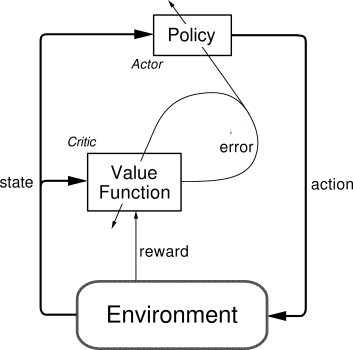
\includegraphics[width=200]{img/actor_critic.png}
\end{center}
\caption[Actor Critic diagram]
{Representation of the Actor Critic interface.}
\label{fig:AC}
\end{figure}

In Figure \ref{fig:AC} you can see how the error is computed based on the approximation of the value function
changing how actor and critic behave.
The hole learning process depend on the error and is defined as the difference between the future returns and
the approximation of this value made by the algorithm.
More formally:
\begin{equation}
    \delta_t=r_{t+1}+\gamma V(s_{t+1})-V(s_t)
\end{equation}
By minimizing this error $\delta_t$ the policy will trend to the optimal policy.
The value function will also approximate more precisely future return values.


\subsection{\aclp{SMDP}}

A \ac{SMDP} is a framework for \newconcept{hierarchical reinforcement learning} in which actions are not atomic, in the sense that they
do not last for just one time step, can be composed by several smaller actions and make decisions based on several states.

This complex actions are named options and can be expressed as a tuple $\langle \mathcal{I}, \pi, \beta \rangle$ where
$\mathcal{I}$ is the set of initial states
where the option is available, $\pi$ is the policy that defines which actions must be taken inside the option and $\beta$ is a
probability distribution over states of the option being interrupted.
More formally, a Markov option is made up by:
\begin{itemize}
    \item $\mathcal{I} \subseteq \mathcal{S}$ where $\mathcal{S}$ is the set of states
    \item $\pi : \mathcal{S} \times \mathcal{A} \rightarrow [0,1]$ where $\mathcal{A}$ is the set of available actions
    during the option, it can also contain other options.
    \item $\beta : \mathcal{S} \rightarrow [0,1]$
\end{itemize}
Since an option can be composed by several actions or other options, and each action lasts one time step, an
option may last more time steps.

%TODO QUITAR ESTO SI NO LO USO
With Markov options the interrupt decision is made on the current state $s_t$ but sometimes we may want to end an option if
some specific amount of time has elapsed.
For this purpose semi-Markov options were created, they use the history of
states and actions taken in that option to select the next action and the end condition.
So in both $\pi$ and $\beta$ instead of
using $\mathcal{S}$ it uses $\Omega$ which is the set of all histories $h_{t\tau}$ defined as follows:
\begin{equation}
    h_{t\tau} = \{s_t,a_t,r_{t+1},s_{t+1},a_{t+1}, ... , r_\tau, s_\tau\}
\end{equation}
Where $\tau$ is the holding time of the option, thus is, the amount of time steps it takes to complete.
Finally the three components of a semi-Markov option are:
$\pi : \Omega \times \mathcal{A} \rightarrow [0,1]$ , $ \beta : \Omega \rightarrow [0,1]$ and
$\mathcal{I} \subseteq \mathcal{S}$

A \ac{SMDP} is a variation of an \ac{MDP} where the set of actions $\mathcal{A}_s$ is made up by semi-Markov options.
A \ac{SMDP} problem can be expressed as a tuple $\left< \mathcal{S}, \mathcal{O}_s, P_o(s,s'), R_o(s),\gamma \right>$ where:
\begin{itemize}
    \item $\mathcal{S}$ is the state space
    \item $\mathcal{O}_s$ is the set of possible options available in state $s$.
    \item $P_o(s,s')$  is the likelihood of reaching state $s' \in \mathcal{S}$ from state $s \in \mathcal{S}$ when taking
    option $o \in \mathcal{O}_s$ , discounted depending on the time taken to reach it.
    \begin{equation}
        P_o(s,s') = \sum_{k=1}^\infty p(s', k) \gamma^k
    \end{equation}
    Where $p(s',k)$ is the probability that the option $o$ terminates in $s'$ after $k$ steps.
    \item $R_o(s)$ is the expected reward for taking option $o$ in state $s$.
    To define it we must introduce $\varepsilon(o,s,t)$ which denotes the event of $o$ being initiated in state $s$ at time $t$.
    \begin{equation}
        R_o(s) = E\left\{ r_{t+1} + \gamma r_{t+2} + \gamma^2 r_{t+3} + \dots
        + \gamma^{k-1} r_{t+k} \;|\; \varepsilon(o,s,t)\right\}
    \end{equation}
    \item $\gamma \in [0,1]$ is the discount factor.
\end{itemize}

With \acp{SMDP} we can define multiple levels of agents where, for example, some of them control basic actions and others
complex options.

\section{\aclp{ANN}}
In this section we describe what are \acfp{ANN},
how they work and which are the most important variants for this thesis.
Most of the definitions and figures are taken from \citetitle{simon2009NN}
by \citet{simon2009NN}

An \ac{ANN} is a collection of artificial neurons that process information in a
parallel way and stores experiential knowledge to use it in another experiences.
It continually adapts connexions between neurons to reach some goals, this process
is named learning.

\subsection{Artificial neuron}
An \newconcept{artificial neuron}, from now on called \newconcept{neuron}, is an
information-processing unit modeled as a mathematical
function with these five basic elements:
\begin{itemize}
    \item A set of connecting links with some weight associated.
    A signal $x_j$ at the input of connexion $j$ related to neuron $k$ is multiplied by the weight $w_{kj}$.
    \item An adder for summing the weighted input signals.
    \item An activation function $\varphi(\cdot)$ that limits the amplitude of the output of a neuron.
    \item A bias $b_k$ which has the effect of increases or reduces the input of the activation function.
    \item An output signal $y_k$ which is the result of the processed information.
\end{itemize}

\begin{figure}[hbtp]
\begin{center}
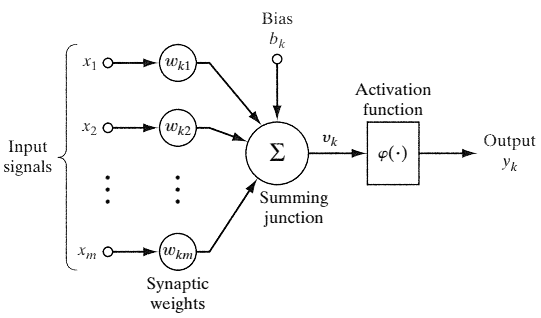
\includegraphics[width=200]{img/artificial_neuron.png}
\end{center}
\caption[Artificial neuron diagram]
{Achitecture of an artificial neuron}
\label{fig:AN}
\end{figure}

In mathematical terms we describe the neuron with the following equation:
\begin{equation}
    y_k=\varphi(b_k+\sum\limits_{j=1}^m w_{kj} x_j)
\end{equation}
where $x_1, x_2, \dots, x_m$ are the input signals;
$w_{k1}, w_{k2}, \dots, wk_m$ are the respective weights of neuron $k$;
$b_k$ is the bias;
$\varphi(\cdot)$ is the activation function;
and $y_k$ is the output signal of the neuron.

\subsection{Multilayer perceptron}
A \newconcept{multilayer perceptron} is a kind of ANN made up by several ordered \newconcept{layers} of neurons.
It is characterized by having an input layer, several hidden layers and an output layer.

The input layer is a set of neurons whose inputs are not connected to other neurons and whose outputs are connected to
the first hidden layer.
Each of the hidden layers satisfies that the output of neurons in layer $i$ is the input of some neurons in layer $i+1$,
except the last hidden layer that is connected with the output layer.
The output layer is a set of neurons whose results form the output signal of the network.
When each neuron has as input all neurons of previous layer the network is named fully connected.

\begin{figure}[hbtp]
\begin{center}
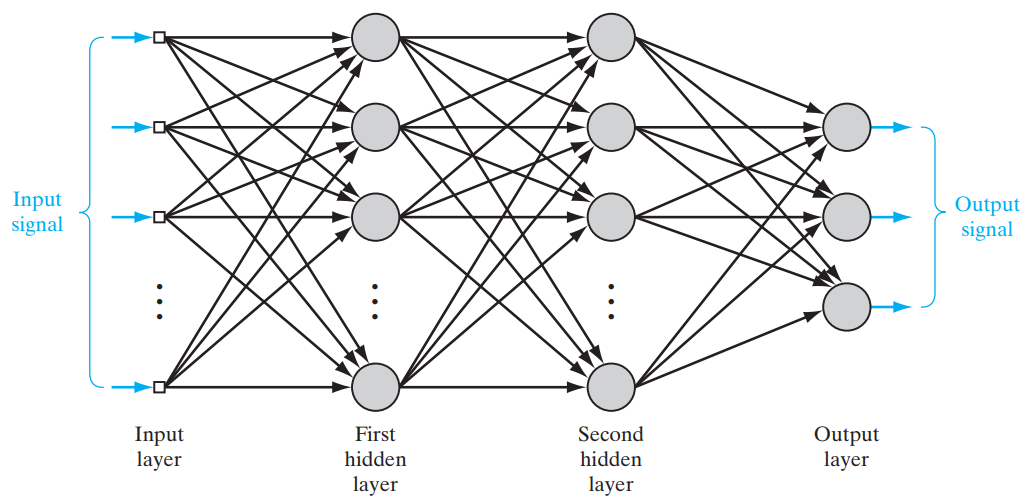
\includegraphics[width=300]{img/multilayer_perceptron.png}
\end{center}
\caption[Multilayer perceptron diagram]
{Fully connected multilayer perceptron.}
\label{fig:FullyMP}
\end{figure}

In multilayer perceptrons there are two kinds of signals, \newconcept{function signals} and \newconcept{error signals}.

A function signal is an input signal that propagates through the network generating an output signal.
The output signal is the result of the function parametrized by all the weights and biases of all neurons.

An error signal originates at the output layer and propagates backwards through the network.
It approximates the difference between the output signal and the desired output signal, given that we are using the \ac{ANN}
to approximate some function.
Each node computes its contribution to the error by estimating the gradient with respect its weights and bias.

The process of adjusting the weights and biases of each neuron to approximate a required output signal given some input
signal is named \newconcept{training}.

Fully connected layers are the most computationally expensive to train because of the amount of connexions and variables.
One way of reducing complexity is to use \newconcept{shared weights}, instead of having different weights for each input of each neuron,
some part of the weights of a neuron are reused to be multiplied for the input of another neurons.
This reduces the number of variables the network should maintain and update, but the number of mathematical computations
will be the same.

Another way of reducing the number of computations is by reducing the number of nodes.
\newconcept{Pooling layers} does that, is a form of non-linear downsampling that applies a function to a group of nodes resuming them
in just one node.

\subsection{Transfer learning in \aclp{NN}}
The aim of \newconcept{transfer learning} techniques is to improve the learning process of a new task given some previous knowledge
about related tasks.
Neural networks, especially the deepest ones, need tons of data to adjust their weights to successfully perform some tasks.

A way to reduce the amount of training data needed and speed up the learning process is to reuse some \ac{NN} previously
trained for a similar task.
Then the \ac{NN} adapts its weights to succeed in the target task.
For example, if we want to recognize dogs inside images, we could use some existing \ac{NN} developed to recognize cats and
then adapt its weights.

Another method is to train our network in a general problem related to the target task to later focus on it.
With deep neural networks we could train a large network on some task and then reuse just the first layers, that should
contain the general feature extraction about the problem.
In the previous example we could take the layers of the network responsible of recognizing shapes and add some new nodes
to train on recognizing dogs.
A simpler example is to train the full network first to recognize shapes and then train on dogs.

\section{\acl{DL}}
\acf{DL} is a machine learning method based on high-level representations of the data.
It basically extends \acp{ANN} by adding multiple hidden layers creating huge neural networks with lots of parameters and interrelations.

In the last years this technique has become really popular as a consequence of its great results comparing to human level performance in many tasks.

\subsection{\acl{CNN}}

This network is a variation of the multilayer perceptron specifically designed to recognize visual patterns.
They are usually made up of four different types of layers: \newconcept{convolutional layers}, \newconcept{ReLU layers},
\newconcept{pooling layers} and fully connected layers.

Convolutional layers apply a convolution to some previous layer, characterized by a filter.
Each node defines its connections based on the filter and their position. The filter is made up by \newconcept{kernel size},
\newconcept{stride}, \newconcept{padding} and \newconcept{values}.
The kernel size defines the shape and amount of nodes of the previous layer that are connected to a convolutional layer node.
The stride defines how the kernel moves across the previous layer, with each move, the filter is applied to some group of
nodes by connecting them to a new node of the convolutional layer.
The padding (specifically zero padding) is the amount of zeros to add around the border of each dimension in the previous
layer, this helps to preserve as much information about the previous layer values.
Finally, the values define the weights for each input signal in each neuron.
These are the same values for each convolutional layer node.
This concept is named \newconcept{shared weights} and minimizes the amount
of variables the neural network has to retain and update.

ReLU layers increases the nonlinear properties of the model by applying the function $f(x)=max(0,x)$ to all outputs of the previous layer.
It is common practice to apply this layer after convolutional layers.
Applying ReLU functions mitigates the \newconcept{vanishing gradient problem}, which is characterized of an exponential
reduction of the gradient through the layers.

Pooling layers generate a downsampled version of the previous layer.
It applies some function ( usually a max function ) to a group of outputs of the previous layer and saves the result in
just one node of the pooling layer.
This technique reduces the parameters of the network which decrease the memory and calculations needed, it also reduces overfitting.

\subsection{\acl{DQN}}
This algorithm was introduced by \citeauthor{mnih2015human} in \citetitle{mnih2015human} (\citeyear{mnih2015human}).

A \acl{DQN}, from now on \ac{DQN}, is a deep convolutional neural network designed to approximate Q values of reinforcement learning.
This agent learns from images to approximate the optimal action-value function (\ffref{subsec:Qlearn}).
The aim of \acp{DQN} is to learn successful policies directly from images of some given problem, for example, a game.
For that purpose the output of the network will be the Q values of each action given some input state.

Bear in mind that when using \acp{NN} in reinforcement learning the learning problem can become unstable or even diverge.
This is caused by the weight updates, that changes not only the result of som action-value pair but all of the action-value associations;
the correlation present in sequence of observations;
and the correlations between the action-values and target values.
For that reason, apart from the \ac{NN}, they used an experience replay ($E$).
This structure saves last $T$ states which the environment has gone by in the format $e_t=(s_t ,a_t , r_t , s_{t+1})$.
Then it picks in an uniformly random manner from this set to train the network.
Training on independent and identically distributed samples helps reducing the instability generated by the neural network.

Q-learning updates are organized in iterations, containing several training steps.
Each iteration has its fixed network
parameters $\theta^-_i$ and applies several training steps obtained from the experience replay to finally change them.
This updates are characterized by the loss applied to the network to adjust its weights.
They defined the loss function in the following way:
\begin{equation}
    L_i(\theta_i)=E_{(s,a,r,s') \sim U(D))} \left [ \bigg(r+\gamma \max_{a'}Q(s',a';\theta_i^-)-Q(s,a;\theta_i)\bigg )^2\right ]
\end{equation}
Where $\theta_i$ and $\theta^-_i$ are the wights of two neural networks with the same architecture.
$\theta_i$ is updated each training step while $\theta^-_i$ only change when the iteration finish, following
$\theta_i = \theta^-_i$ after this happens.

This network has successfully surpass human-level skills in many atari games.
But in montezuma's revenge it was unable to obtain any score.

\subsection{\acl{A3C}\label{subsec:A3C}}
The algorithm \acl{A3C}, from now on \ac{A3C}, was introduced by \citeauthor{mnih2016A3C} in
\citetitle{mnih2016A3C} (\citeyear{mnih2016A3C}).

The main difference between asynchronous methods and the methodology used in \ac{DQN} is the experience replay.
In \ac{A3C} instead of having an experience replay, to take uniformly random states and avoid instability, it runs in
parallel multiple instances of the environment.
At each time step the agent is being trained with different states of multiple environments that runs in isolation.

Another difference between \ac{DQN} and \ac{A3C} is the reinforcement learning approach.
It uses the actor-critic interface introduced in \ffref{subsec:AC}.
It defines two \acp{NN} that represent the value of the state ($V$) and the policy ($\pi$).
$V$ is the output of just one node, but $\pi$ is the output of a set of nodes, each one representing the probability of taking
an action.
In practice this two \acp{NN} share almost all the layers, except the last one ($V$ and $\pi$).

%TODO A LO MEJOR HAY QUE DEFINIR N-STEP RETURNS EN ESE APARTADO
Also the loss function used to train the network differ from \ac{DQN}, it uses n-step returns (\ffref{subsec:returns}) and it does not
update $Q$ values, it updates $V$ and $\pi$.
The number of steps used in the loss function is $t_{max}$ ( an hyperparameter ) but if a
final state is reached before that, the loss is computed with less than $t_{max}$.
It also adds an entropy factor $H$ based on the policy, in order to improve exploration by discouraging premature
convergence to suboptimal deterministic policies.
\ac{A3C} uses the following update function:
\begin{equation}
    \nabla_{\theta'}\;log\:\pi(a_t\mid s_t;\theta')\;A(s_t,a_t;\theta,\theta_v)+\beta\nabla_{\theta'}H(\pi(s_t;\theta'))
\end{equation}
Where $A$ is the advantage function of n-step returns in terms of $V$.
$\theta'$ are the weights related to the policy and $\theta_v$ the weights related to the value function.
$\beta$ is an hyperparameter that controls the strength of the entropy regularization term.
The advantage function defines at follows:
\begin{equation}
    A_t=\sum^{k-1}_{i=0}\gamma^i r_{t+i}+\gamma^k V(s_{t+k};\theta_v)-V(s_t;\theta_v)
\end{equation}
Where $k$ can vary from state to state ( if a final state is reached ) and is upper-bounded by $t_{max}$.

This algorithm is parallelized in different threads which contain different replicas of a shared \ac{NN}.
Each thread interacts with the environment using his own \ac{NN}, until $t_{max}$ or end of game are reached, and updates the
global network parameters with the update function above.
The algorithm used in each thread is the following.

\begin{algorithm}[hbtp]
\begin{algorithmic}
    \State \newconcept{//Assume global shared parameter vectors $\theta$ and $\theta_v$ and global shared counter $T = 0$}
    \State \newconcept{//Assume thread-specific parameter vectors $\theta' and \theta_v'$}
    \State Initialize thread step counter $t \leftarrow 1$
    \Repeat
        \State Reset gradients: $d\theta \leftarrow 0$ and $d\theta_v \leftarrow 0$.
        \State Synchronize thread-specific parameters $\theta' = \theta$ and $\theta_v' = \theta_v$
        \State $t_{start} = t$
        \State Get state $s_t$
        \Repeat
            \State Perform $a_t$ according to policy $\pi(a_t|s_t;\theta')$
            \State Receive reward $r_t$ and new state $s_{t+1}$
            \State $t \leftarrow t + 1$
            \State $T \leftarrow T + 1$
        \Until{terminal $s_t $ \textbf{or} $t-t_{start} == t_{max}$ }
        \State R = \begin{cases}
                0,   & \text{ for terminal }\ s_t \\
                V(s_t, \theta_v'),   & \text{for non-terminal } s_t \;\newconcept{// Bootstrap from last state}\\
            \end{cases}
        \For{ $i \in \{ t-1,\dots,t_{start}\}$}
            \State $R \leftarrow r_i + \gamma R$
            \State Accumulate gradients wrt $\theta': d\theta \leftarrow d\theta + \nabla_{\theta'} log\:\pi(a_i\mid s_i;\theta')(R-V(s_i;\theta_v'))+\beta\nabla_{\theta'}H(\pi(s_i;\theta'))$
            \State Accumulate gradients wrt $\theta_v': d\theta_v \leftarrow d\theta_v + \partial(R-V(s_i;\theta_v'))^2 / \partial \theta_{v}'$
        \EndFor
        \State Perform asynchronous update of $\theta$ using $d\theta$ and of $\theta_v$ using $d\theta_v$.
    \Until{$T > T_{max}$}
\end{algorithmic}
\caption{\acl{A3C} - psudocode for each actor-learner thread (\cite{mnih2016A3C})}
\label{alg:A3C}
\end{algorithm}


%%% Local Variables:
%%% mode: latex
%%% TeX-master: "../report"
%%% End:

\cleardoublepage
\chapter{Methodology}

\section{Algorithms}

We have modified the \ac{A3C} algorithm in order to take advantage of sub-tasks with the purpose of enhancing training speed
and exploration.
We refer to this new algorithm as \acf{MA3C} and in this section it can be found specifications about the architectures of
both \acp{ANN}: \ac{A3C} and \ac{MA3C}.
In addition we will explain the \ac{MA3C} algorithm.

They have been developed using tensorflow (\cite{tensorflow2015}), an open source machine learning framework which the authors
of \ac{A3C} and \ac{DQN} are also using (\cite{deepmind_tensorflow}).

\subsection{\acl{A3C}\label{subsec:AlgorithmA3C}}

As we have explained before (\ffref{subsec:A3C}), this algorithm uses the image of the environment to represent the state.
We have used almost the same preprocessing and network architecture (\ffref{fig:A3C}) than in \citetitle{mnih2016A3C} (\cite{mnih2016A3C}).
In practice, the images of any game are resized to $84 \times 84$ greyscale pixels in order to reduce the computational cost of training and to fit the convolutions.
The algorithm applies this preprocessing to 4 stacked frames allowing the \ac{ANN} to implicitly calculate the movement
of the different pixels/objects on the screen.
There is a frame skip of 4, which means that, only one out of four consecutive frames is taken into account and stacked.
There is also a component-wise maximum selection over two consecutive frames, the one stacked and the next one which will
not be stacked.
The state dimensionality is $84 \times 84 \times 4$ which defines the input layer of the \ac{CNN}.
This is just for Atari games, in Simple States (\ffref{subsec:SimpleStates}) and Complex States (\ffref{subsec:ComplexStates})
the RGB channels of a single frame are used instead.
The dimensionality of the input layer in that games is $84 \times 84 \times 3$.

There are several hidden layers specifically designed to obtain high level abstractions of the environment frames.
The first one is a convolutional layer (\ffref{subsec:CNN}) with $16$ filters with kernel dimension $8 \times 8$ and stride $4$,
followed by a \ac{ReLU} layer.
The second layer is also a convolutional layer, but with $32$ filters with kernel dimension $4 \times 4$ and stride 2,
again followed by a \ac{ReLU} layer.
The last hidden layer intends to represent general features about the state of the game.
It is a fully connected composed by 256 ReLU nodes.

From these 256 features the actor and critic layers, which are the output layers, decide the actions that should be taken
in order to maximize the reward, as explained in (\ffref{subsec:AC}).
The actor is made up by as many nodes as actions available in each game with values from $0$ to $1$, representing the
probability distribution $\pi$.
The critic is just $1$ neuron representing the value function $V(s_t)$.

\begin{figure}[hbtp]
\begin{center}
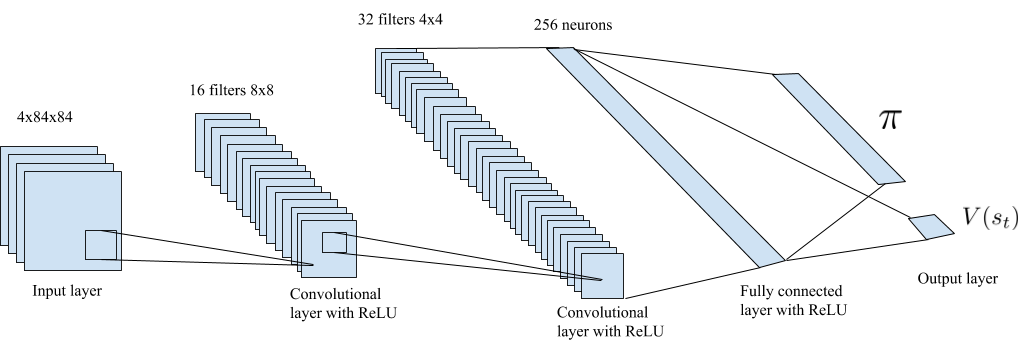
\includegraphics[width=430]{img/A3C_architecture.png}
\end{center}
\caption[A3C architecture]
{Architecture of the \ac{A3C} algorithm.}
\label{fig:A3C}
\end{figure}

\subsection{\acl{MA3C}\label{subsec:MA3C}}

This algorithm is strongly associated with hierarchial reinforcement learning, since the last layer of \ac{A3C}
($\pi$ and $V(s_t)$) is replicated several times in order to model different tasks inside a common bigger problem.

\begin{figure}[hbtp]
\begin{center}
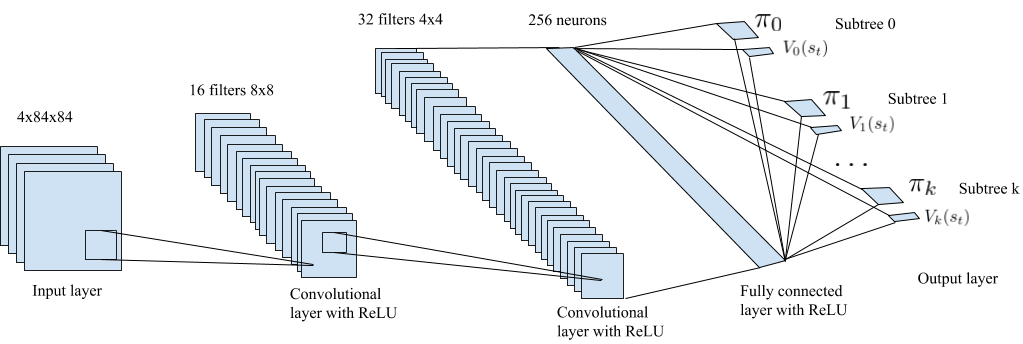
\includegraphics[width=430]{img/MA3C_architecture.png}
\end{center}
\caption[MA3C architecture]
{Architecture of the \ac{MA3C} algorithm.}
\label{fig:MA3C}
\end{figure}

As we can see in \ffref{fig:MA3C} the architecture is very similar to \ac{A3C}.
There is an input layer of size $84 \times 84 \times 4$, a convolutional layer with $16\; 8 \times 8$ filters, another
convolutional layer with $32 \; 4 \times 4$ filters and a fully connected layer with $256$ nodes.
The output layer is made up by $K$ copies of the \ac{A3C} output layer, where $K = k-1$ is an hyperparameter which might be
different depending on the use case.
For each of the games we have set $K$ to a different value: with Simple States we have used $K=3$, with Complex States
$K=2$ and with \ac{MR} $K=4$.
The first two depend on the number of phases (see \ffref{subsec:SimpleStates} and \ffref{subsec:ComplexStates}) and the last one
depends on the number of intermediate rewards (see \ffref{subsec:MontezumasRevenge}).

The architecture of \ac{MA3C} contains multiple \newconcept{subtrees} defining different \acl{AC} approaches to the given input state,
each one connected to the high level features (last layer) but not between them.
With this architecture the algorithm uses transfer learning (\ffref{subsec:TransferLearning}) to extract common features
about the environment, which are useful for all \ac{AC} layers.
When some task is already trained and a new one starts to train, most of the network is reused, speeding up the learning
process.
Given that every subtree is used to solve a different task inside a bigger problem, the common parameters will be optimized to
extract as much information as possible about the general problem, while the weights of each subtree will be optimized to
succeed in the specific task.

The update function, advantage function and algorithm of \ac{MA3C} remain the same ones as in \ac{A3C} (\ffref{subsec:A3C}).
The only difference is that this one selects the chunk of the parameter vectors $\theta'$ and $\theta_{v}'$ that will be updated
depending on the currently active subtree.
The method which selects one subtree or another is arbitrary, they might be selected with an \ac{AI} method, just
with a couple of rules or be given by the state.
For this thesis we have used two approaches: part of the state, in Simple States (\ffref{subsec:SimpleStates}) and Complex States
(\ffref{subsec:ComplexStates}); and some rules about the position of the hero in Montezuma's Revenge (\ffref{subsec:MontezumasRevenge}).

The full modified algorithm is shown in \ffref{alg:MA3C}.

\begin{algorithm}[hbtp]
\begin{algorithmic}
    \State \newconcept{//Assume global shared parameter vectors $\theta$ and $\theta_v$ and global shared counter $T = 0$}
    \State \newconcept{//Assume thread-specific parameter vectors $\theta' and \theta_v'$}
    \State \newconcept{//Assume subree-specific parameter vectors $\theta'^k and \theta_v'^k$ from $\theta' and \theta_v'$}
    \State Initialize thread step counter $t \leftarrow 1$
    \Repeat
        \State Reset gradients: $d\theta \leftarrow 0$ and $d\theta_v \leftarrow 0$.
        \State Synchronize thread-specific parameters $\theta' = \theta$ and $\theta_v' = \theta_v$
        \State $t_{start} = t$
        \State Get state $s_t$
        \Repeat
            \State Perform $a_t$ according to policy $\pi(a_t|s_t;\theta')$
            \State Receive reward $r_t$ and new state $s_{t+1}$
            \State $t \leftarrow t + 1$
            \State $T \leftarrow T + 1$
        \Until{terminal $s_t $ \textbf{or} $t-t_{start} == t_{max}$ }
        \State R = \begin{cases}
                0,   & \text{ for terminal }\ s_t \\
                V(s_t, \theta_v'),   & \text{for non-terminal } s_t \;\newconcept{// Bootstrap from last state}\\
            \end{cases}
        \For{ $i \in \{ t-1,\dots,t_{start}\}$}
            \State $R \leftarrow r_i + \gamma R$
            \State Select $k$ \;\newconcept{// Select subtree with any criteria}
            \State Accumulate gradients wrt $\theta'^k: d\theta \leftarrow d\theta + \nabla_{\theta'} log\:\pi(a_i\mid s_i;\theta')(R-V(s_i;\theta_v'))+\eta\nabla_{\theta'}H(\pi(s_i;\theta'))$
            \State Accumulate gradients wrt $\theta_v'^k: d\theta_v \leftarrow d\theta_v + \partial(R-V(s_i;\theta_v'))^2 / \partial \theta_{v}'$
        \EndFor
        \State Perform asynchronous update of $\theta$ using $d\theta$ and of $\theta_v$ using $d\theta_v$.
    \Until{$T > T_{max}$}
\end{algorithmic}
\caption{\acl{MA3C} - psudocode for each actor-learner thread (\cite{mnih2016A3C})}
\label{alg:MA3C}
\end{algorithm}

\section{Environments}

In order to demonstrate the capabilities of \ac{MA3C} over \ac{A3C} we have developed two simple environments where the
weaknesses of the second one come to light.
We have also compared the algorithms in a real game, \acl{MR}, which has become famous because of its difficulty.

These three environments have been used through a useful toolkit called OpenAi Gym (\cite{gym}), in which the different games
can be accessed by a common interface facilitating the analysis of different algorithms and games.


\subsection{Simple States\label{subsec:SimpleStates}}

This game is made by a $6 \times 10$ grid of square blocks.
Their colors define the kind of object and how they will interact with the hero (an special object).
This are the different types:
\begin{itemize}
  \item \newconcept{hero}: A block that can be controlled by the actions.
  \item \newconcept{wall}: If the hero hits a wall the game ends and he obtains a reward of value -1.
  When this happens we say that the hero dies.
  \item \newconcept{checkpoint}: When the hero reach this object he obtains a reward of value 1 and enables the hidden
  checkpoint reward.
  Once the hero reaches it for the first time he will never obtain the reward again.
  \item \newconcept{hidden checkpoint}: When the hero reach this object enables the door.
  It basically forces the hero to pass and there is no reward when this happens.
  \item \newconcept{door}: If the hero reach the door having gone through the different checkpoints the game ends and
  he obtains a reward of value 1.
\end{itemize}

\begin{figure}[hbtp]
\begin{center}
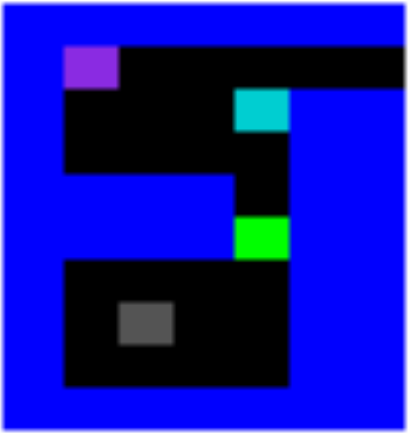
\includegraphics[width=200]{img/SimpleStates_going_up.png}
\end{center}
\caption[Simple States game]
{The hero navigating through a hostile environment trying to reach the door. The wall, hero, checkpoint, hidden checkpoint
and door are represented with the following colors respectively: blue, grey, green, turquoise and violet.}
\label{fig:SimpleStates}
\end{figure}

The goal of the hero is to reach the door by passing through the different checkpoints without colliding
with any wall, this will give to the hero the maximum score, 2 points.
The game is organized in three different phases/states, each one having a different objective.
The first one's objective is to reach the checkpoint,
of the second one's, the hidden checkpoint and the third one's, the door.
The information about the current phase is allways available to the player.

In order to solve this game with both \ac{A3C} and \ac{MA3C} algorithms we must model it as a \ac{SMDP} problem,
describing components of the tuple $\langle\mathcal{S}, \mathcal{A}_s, \mathcal{P}_a(s,s'), \mathcal{R}_a(s,s'), \gamma \rangle$.

\begin{itemize}
    \item Each states is a pair $s_t = (\mathbf{F}, p)$ where $p \in \{0,1,2\}$ is the phase of the game and
    $\mathbf{F}$ is the matrix of RGB pixels with dimensionality $84\times84\times3$.
    $\mathcal{S}$ is the set of all $s$ which satisfies the conditions about object collisions presented above.

    \item $\forall s \; \mathcal{A}_s = \{\textsc{UP}, \textsc{DOWN}, \textsc{LEFT}, \textsc{RIGHT}, \textsc{WAIT}\}$ and each action $a_{t}\in \mathcal{A}_s $ corresponds to
    the movement of the hero.

    \item This game is deterministic, which means that $\forall s\forall a\exists s' \; |\; \mathcal{P}_a(s,s') = 1$ implying
    $\forall s\forall a\forall {s''\neq s'} \;\; \mathcal{P}_a(s,s'') = 0$

    \item The reward function is determined as explained before.
    Depending on the phase ($p$) some transition from a frame $\mathbf{F}_t$
    to another frame $\mathbf{F}_{t+1}$ may come with a reward $\mathcal{R} \in \{ -1, 0, 1\}$.

    \item The discount factor $\gamma$ is $0.99$
\end{itemize}

The purpose of creating this game is to prove that the \ac{MA3C} algorithm (\ffref{subsec:MA3C}) has better exploration
skills than A3C (\ffref{subsec:A3C}).

% TODO F PONER QUE CUMPLE LA MARKOV PROPERTY?
\subsection{Complex States\label{subsec:ComplexStates}}

This game is really similar to the previous one but the dynamics are a bit different.
The hero must follow a series of steps to reach the door.
The order in which the hero must go through the objects is: checkpoint $\rightarrow$ hidden checkpoint $\rightarrow$
door $\rightarrow$ hidden checkpoint $\rightarrow$ checkpoint $\rightarrow$ door.
We force the hero to go back on his own steps when he reaches the door.
In this game some of the rewards also change.
These are the changes with respect to the Simple States game, the rest remains equal:
\begin{itemize}
    \item \newconcept{checkpoint}: The first time that the hero goes through this object he obtains a reward of 1.
    Then he must follow the rest of the path described above to obtain again 1 of score (after the second time he visits the hidden checkpoint).
    \item \newconcept{hidden checkpoint}: In this game both 2 times that the hero goes through this object
    (following the path) receives 1 of score.
    The first time the checkpoint object enables the reward and the second time the door enables it.
    \item \newconcept{door}: The first time the hero reach the door it moves to the starting position of the hero (bottom left corner)
    and gives him 1 of score.
    The second time behaves as in Simple States.
\end{itemize}

\begin{figure}[hbtp]
\begin{center}

\includegraphics[width=200]{img/ComplexStates_going_back.png}
\end{center}
\caption[Complex States game]
{The hero after reaching the door for first time. The wall, hero, checkpoint, hidden checkpoint
and door are represented with the following colors respectively: blue, grey, green, turquoise and violet.}
\label{fig:ComplexStates}
\end{figure}


In this game there are only two phases.
The first one goes from the start until the first time the hero reaches the door.
The second one finishes the second time it reaches the door.
As in Simple States the hero must follow the path in order to obtain the rewards and finish the game.
The information about the current phase is also available to the player.

The \ac{MDP} problem of this game is exactly the same as in Simple States (\ffref{subsec:SimpleStates}).
The only thing that changes are the rules of rewards and phases which we have already defined.

The purpose of creating this game is to prove that \ac{A3C} is quite bad going back on his own steps (when the image of the
game is similar) while for \ac{MA3C} is easy.

\subsection{Montezuma's Revenge\label{subsec:MontezumasRevenge}}

We wanted to test \ac{MA3C} in an environment which other authors also did a research on.
\acf{MR} is an Atari game created in 1984 which recently has become famous because of its difficulty.
\ac{DQN} and \ac{A3C} algorithms get less than $100$ score on average when playing this game (\cite{mnih2016A3C}).

The hero, Panama Joe, goes into an Aztec pyramid full of treasures, traps and monsters.
The game takes place inside the pyramid where there are different rooms with the treasures he must collect.
In order to navigate from a room to another he must collect keys and open doors while avoiding traps and monsters.
It is a relatively big game (24 rooms) where the agent starts in screen 1 (\ffref{fig:MontezumasRevenge}) and must navigate
through most of the rooms in order to collect a group of special gems which make him win the game.

\begin{figure}[hbtp]
\begin{center}
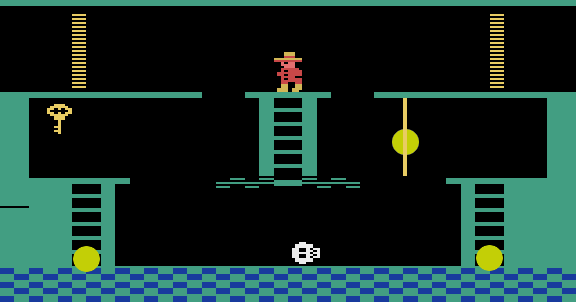
\includegraphics[width=300]{img/montezuma_checkpoints.png}
\end{center}
\caption[Montezuma's Revenge game]
{The hero is in the starting position of the game, in the first screen of \acl{MR}.
Three yellow bullets have been added in order to represent the checkpoints.}
\label{fig:MontezumasRevenge}
\end{figure}

Since this game is really complex and computationally expensive to train, we have made some changes to it.
\begin{itemize}
    \item In the hole game there are several screens but we will only use the first one in my experiments.
    \item The hero has multiple lives but we will consider he has just $1$ and, if he dies, the game will be reset.
    \item When the hero reaches the key we will also reset the game, so the unique goal of the hero is to take that object.
\end{itemize}
Nevertheless, the procedures remain the same as in the original game.

At each time step, the player can take 8 different actions: \textsc{Noop} (stay
still), \textsc{Fire} (jump straight up), \textsc{Up}, \textsc{Right},
\textsc{Left}, \textsc{Down}, \textsc{LeftFire} (jump to the left),
\textsc{RightFire}.

There are one rope and three stairs with which the hero can go up and down.
If he jumps into the rope he will grab the cord, but ,if he jumps into the stairs, this will not happen.
From now on we will refer to the right stairs as \newconcept{Rstairs} and to left ones \newconcept{Lstairs}.
We will use later the position (in screen space) of the objects, which are the following:
\begin{itemize}
    \item rope: from $(109, 174)$ to $(109, 212)$
    \item Rstairs: $(133, 148)$
    \item Lstairs: $(21, 148)$
    \item key: $(14, 209)$
\end{itemize}
In order to obtain this positions, and the agent's position, we have used the memory layout described in \citetitle{adriaTFG}
(\cite{adriaTFG}).

The hero can die within two manners: by falling into the floor from some high position (e.g. from the rope) or by touching the skull in the bottom, which is always moving left and right.

The hero can obtain a score by collecting the key, which gives him 100 points.
He can also win 10 points by passing through each of the checkpoints which we have manually added to guide the agent
towards the key.
Since they have been selected in order to guide the agent towards $\pi^*$ this is a way of applying reward shaping
(\ffref{subsec:RewardShaping}) to Montezuma's Revenge.
The potential function $\phi(s)$ is defined in the following way:
\begin{equation}
    \State \phi(s) = \begin{cases}
                 10, & \text{hero visits for the first time the positions: rope, Rstairs, Lstairs, key} \\
                 0,  & \text{otherwise} \\
            \end{cases}
\end{equation}

The difficulty is due to the facility to die and the remoteness of the rewards.

We have modeled this game as a \ac{SMDP} (\ffref{subsec:SMDP}),
with the tuple $\left< \mathcal{S}, \mathcal{O}_s, P_o(s,s'), R_o(s),\gamma \right>$.

The state $s \in \mathcal{S}$ is a pair $s_t = (\mathbf{F}, p)$ where $p \in \{0,1,2,3\}$ is the phase/option of the game and
$\mathbf{F}$ is the matrix of processed pixels (as described in \ffref{subsec:AlgorithmA3C}).

The different phases are described by consecutive options in which $\mathcal{I}$ and $\beta$ are specified, but $\pi$
must be learned by the algorithm.
The consecutive options, in order of appearance, are the following:
\begin{itemize}
    \item $o_0$ is the option defined by $\mathcal{I} = {s_0}$, the game initial state, and
    $\beta$ being:
    \begin{equation}
    \State \beta = \begin{cases}
                 1, & \forall s \in \mathcal{S}_{rope} \\
                 0,  & \forall s \notin \mathcal{S}_{rope} \\
            \end{cases}
    \end{equation}
    Where $\mathcal{S}_{rope}$ is the set of states in which the agent is in the same screen space as the rope.

    \item $o_1$ is the option defined by $\mathcal{I} = \mathcal{S}_{rope}$ and
    $\beta$ being:
    \begin{equation}
    \State \beta = \begin{cases}
                 1, & \forall s \in \mathcal{S}_{Rstairs} \\
                 0,  & \forall s \notin \mathcal{S}_{Rstairs} \\
            \end{cases}
    \end{equation}
    Where $\mathcal{S}_{Rstairs}$ is the set of states in which the agent is in the same screen space as the Rstairs.

    \item $o_2$ is the option defined by $\mathcal{I} = \mathcal{S}_{Rstairs}$ and
    $\beta$ being:
    \begin{equation}
    \State \beta = \begin{cases}
                 1, & \forall s \in \mathcal{S}_{Lstairs} \\
                 0,  & \forall s \notin \mathcal{S}_{Lstairs} \\
            \end{cases}
    \end{equation}
    Where $\mathcal{S}_{Lstairs}$ is the set of states in which the agent is in the same screen space as the Lstairs.

    \item $o_3$ is the option defined by $\mathcal{I} = \mathcal{S}_{Lstairs}$ and
    $\beta$ being:
    \begin{equation}
    \State \beta = \begin{cases}
                 1, & \forall s \in \mathcal{S}_{key} \\
                 0,  & \forall s \notin \mathcal{S}_{key} \\
            \end{cases}
    \end{equation}
    Where $\mathcal{S}_{key}$ is the set of states in which the agent is in the same screen space as the rope.
    Bear in mind that $\beta$ is defined in a way that the option finishes in the same states as the game does.
\end{itemize}
The action set available inside each option is
$\mathcal{A}_s = \{\textsc{Noop}, \textsc{Fire}, \textsc{Up}, \textsc{Right}, \textsc{Left},$
$\textsc{Down}, \textsc{LeftFire}, \textsc{RightFire}\}$.
By defining the options in this way, we divide the problem in 4 phases from which, once
it changes to the next, it is impossible to go back to another previous option/phase.
This simplifies the game, being really similar to Simple States and Complex States games.

As far as the agent will learn how to act inside the option, we cannot accurately define $ P_o(s,s') $ and $ R_o(s) $.
This is because the number of steps $k$ depends on the policy of the option.
But we can say that options $o_0, o_1$ and $o_2$ have a reward $r_{t+k} = 10$ while $o_3$ has a reward $r_{t+k} = 110$,
i.e., the score given by the key and by the checkpoint.

The discount factor $\gamma$ is $0.99$.

We have decided to model this problem as a \ac{SMDP} in order to expose the strengths of \ac{MA3C} inside hierarchical
learning models, in the knowledge that modeling it as a \ac{MDP} may have been easier and makes more sense.


%%% Local Variables: 
%%% mode: latex
%%% TeX-master: "../report"
%%% End: 

\cleardoublepage
\chapter{Evaluation}

In this chapter we will supply enough evidence about how the \ac{MA3C} algorithm learns faster and explores better than
\ac{A3C} in environments where subgoals can be defined.

All the code needed to make the following analysis was developed inside a project of the Universidad Pompeu Fabra researcher
Miquel Juyent.
The \ac{A3C} algorithm was fully provided by him while the algorithm \ac{MA3C} and the games Simple States and Complex
States have been developed by us.
The seed to initialize the weights of the different networks where randomly chosen in each of the experiments and runs.

We have used multiple common hyperparameters along the three experiments, which are:
\begin{itemize}
    \item The discount factor $\gamma = 0.99$ (\ffref{subsec:returns}).
    \item $t_{max}=20$ (\ffref{subsec:A3C}).
    \item Entropy regularization term $\eta = 0.1$ (\ffref{subsec:A3C}).
    \item Value regularization term $ \rho = 0.5$ (\ffref{subsec:A3C}).
    \item The learning rate is $0.007$ (\ffref{subsec:multilayer-perceptron}).
\end{itemize}

\section{Simple States}

We have compared the performance of both algorithms \ac{A3C} (\ffref{alg:A3C}) and \ac{MA3C} (\ffref{alg:MA3C}) in Simple
States game (\ffref{subsec:SimpleStates}).

The specific hyperparameters used in this experiment which differ from the general ones are:
\begin{itemize}
    \item The number of threads in which the algorithms have been parallelized is $8$ (\ffref{subsec:A3C}).
    \item Subtrees $K = 3$ (just for \ac{MA3C}, \ffref{subsec:MA3C}).
\end{itemize}


This parameters have been chosen in order to show the disadvantages of \ac{A3C} as opposed to \ac{MA3C}.
There might be a different combination of hyperparameters in which, at the end, both algorithms converge to the same solution.
Since the ultimate goal is to show how \ac{MA3C} explores better, this hyperparameters are good enough.

\begin{figure}[hbtp]
\begin{center}
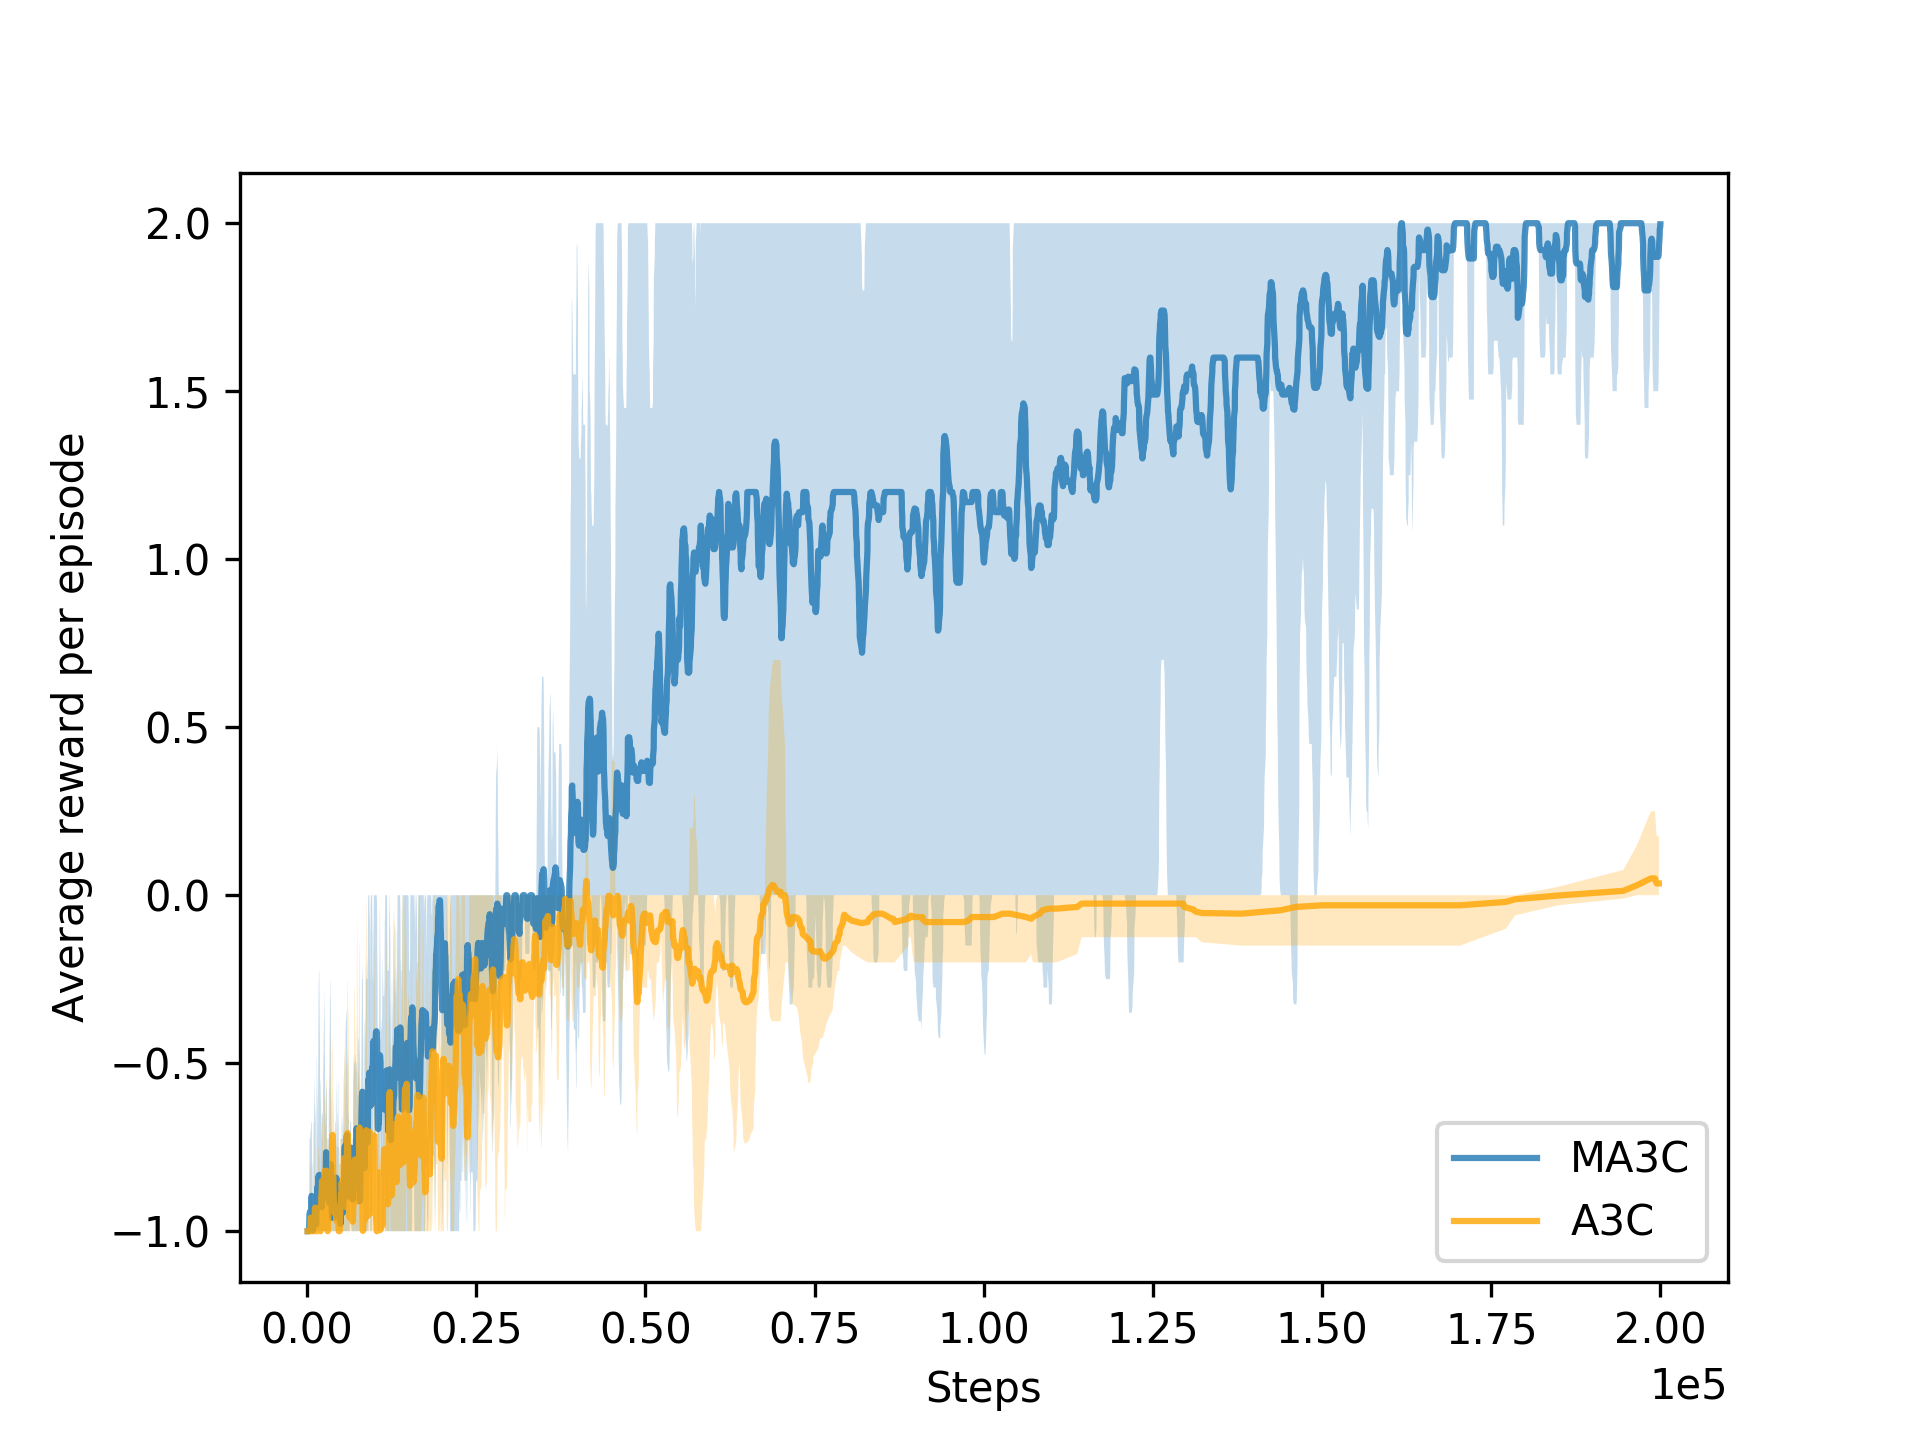
\includegraphics[width=250]{img/SimpleStates_performance.png}
\end{center}
\caption[Simple States performance]
{Average score over $5$ runs of \ac{A3C} and \ac{MA3C} algorithms in Simple States environment (200k steps/actions).
The graphics have been smoothed by a moving average with a $20$ steps window.
The shadow represents maximum and minimum values of those $5$ smoothed runs.}
\label{fig:SimpleStates_performance}
\end{figure}

The learning process of both algorithms measured by score over steps is shown in \ffref{fig:SimpleStates_performance}.
As can be seen, \ac{MA3C} algorithm obtains score $2$ (checkpoint and door) while \ac{A3C} obtains score $0$ because it
reaches the checkpoint but then hits a wall.

This is due to the subtree changes which the algorithm makes every time it goes through any of the checkpoints (normal
and hidden).
Every time the change happens the data in the common network changes in a different manner (the direction of the gradient) %TODO R NO HE HABLADO DEL GRADIENTE , QUITAR?
until it converges to common features for all subtrees.
Thanks to that, the randomness is implicitly increased every time the change happens until convergence is achieved.
And, as far as more random actions lead to better exploration, this algorithm is using the subgoals (checkpoints) in
order to enhance exploration only when needed, specifically when a new phase is achieved.

It is important to remember that the hidden checkpoint does not give any reward, so in some cases there will be no need
of adding intermediate rewards, just subtree changes.
In general, when solving a problem with \ac{MA3C} it might be no need of doing reward shaping (\ffref{subsec:RewardShaping})
and carefully select the $\mathcal{F}$ function to ensure near-optimal policies.
The subtree changes can be done in any state and the optimal policies will remain the same, it will just enhance exploration
after reaching that states.

\section{Complex States}

Thanks to the results obtained with Simple States game, we realized that \ac{MA3C} may be better than \ac{A3C} learning
different policies from two really similar states.
We decided to test the algorithms in this game (Complex States, \ffref{subsec:ComplexStates}) in order to observe how they
behave in environments in which it is mandatory to retrace its steps.
It is important to mention that in this game there is no hidden checkpoint, so the \ac{MA3C} does not have as much
``advantage" as in Simple States.

The specific hyperparameters used in this experiment which differ from the general ones are:
\begin{itemize}
    \item The number of threads in which the algorithms have been parallelized is $8$.
    \item Subtrees $K = 2$. (just for \ac{MA3C})
\end{itemize}

\begin{figure}[hbtp]
\begin{center}
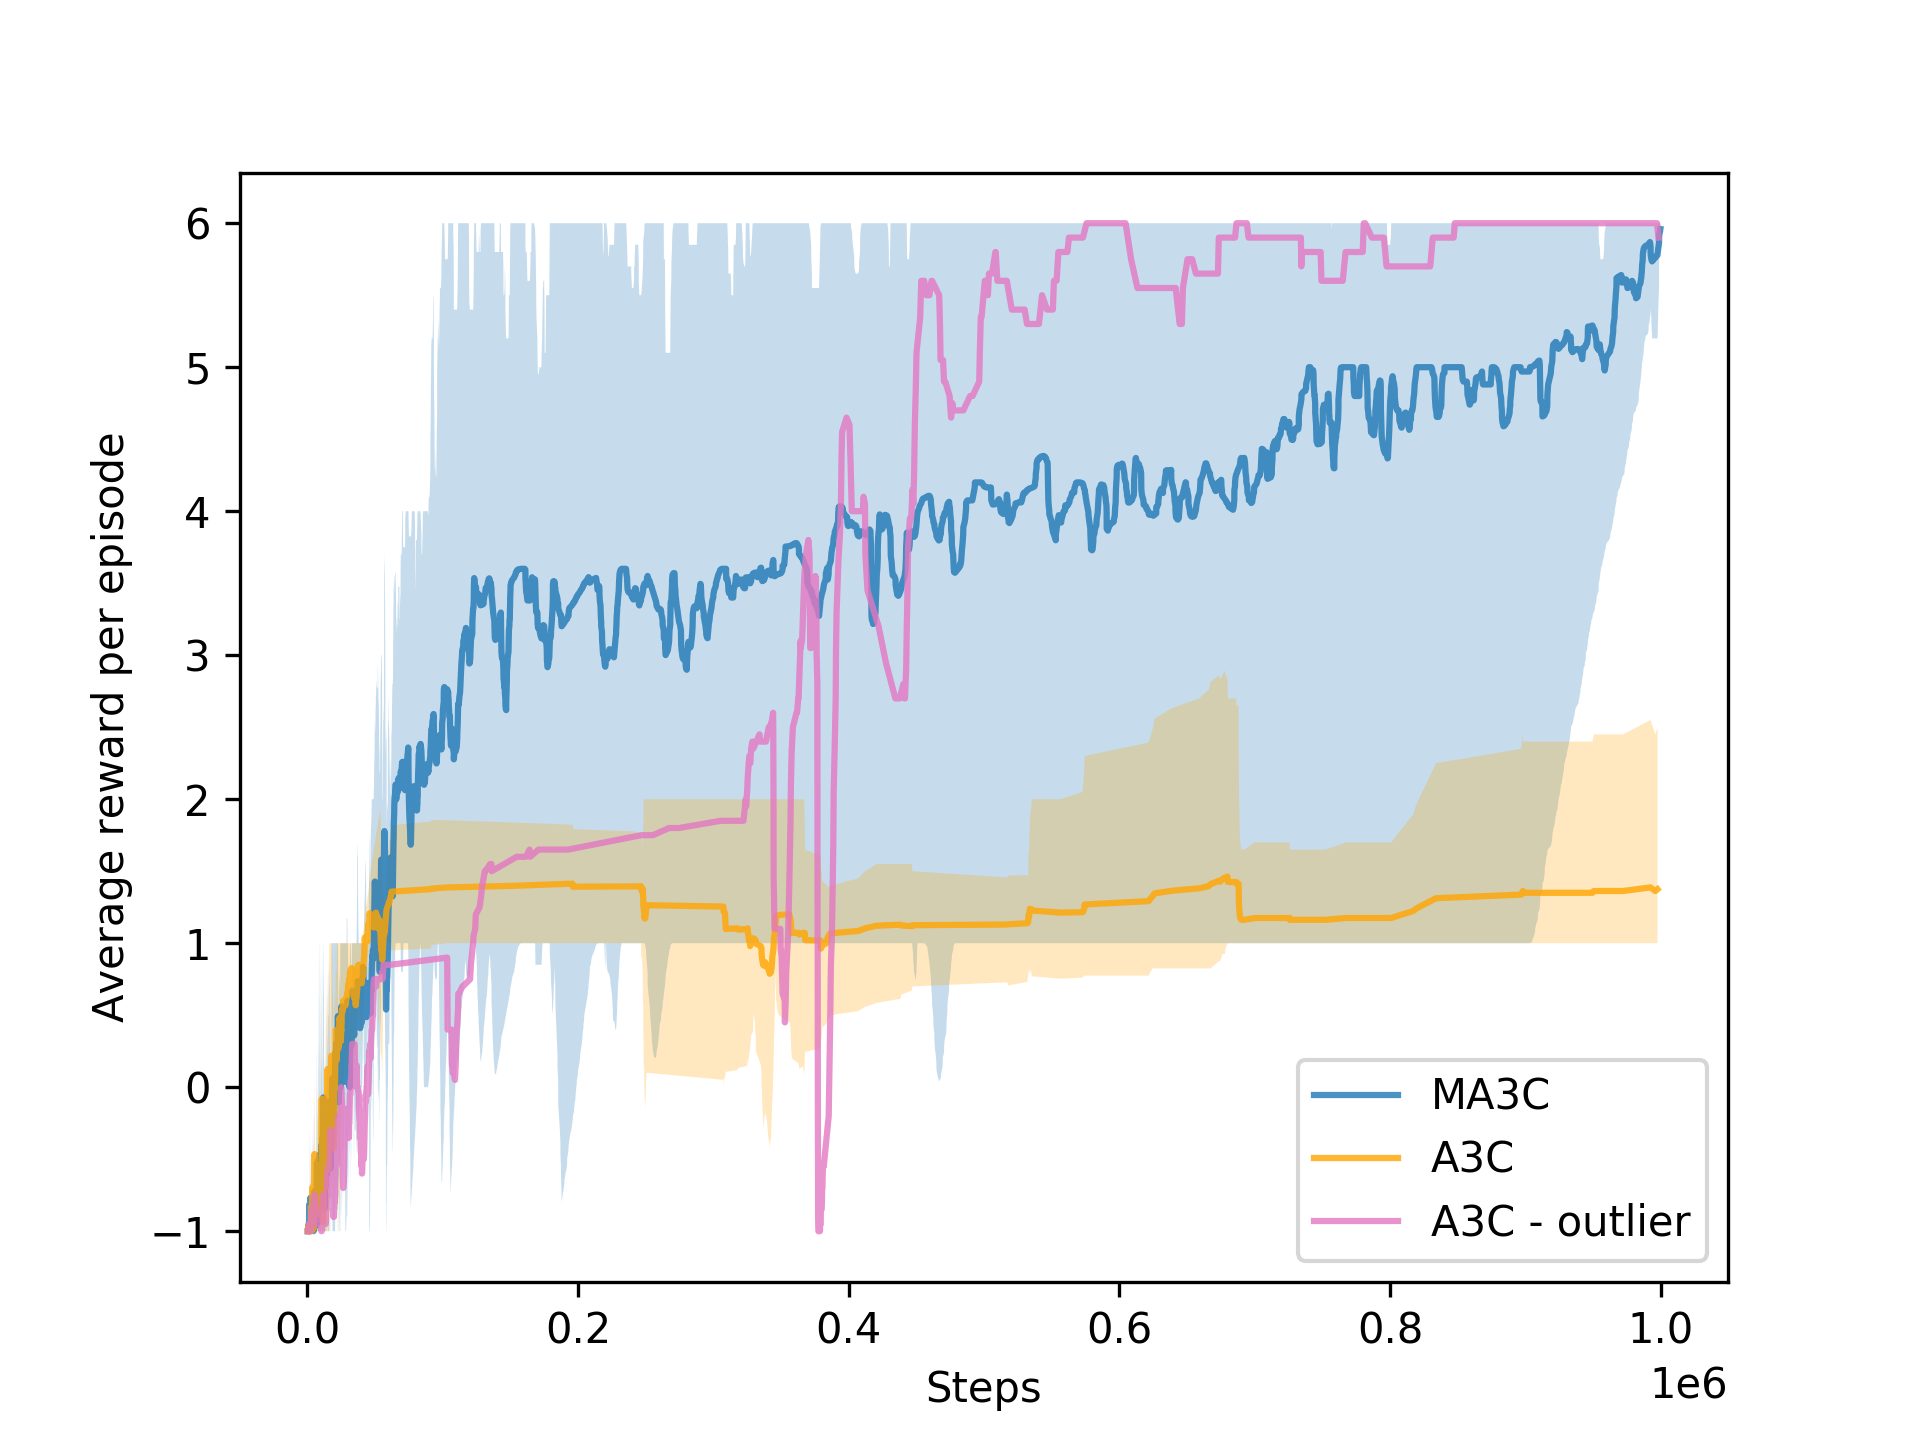
\includegraphics[width=250]{img/ComplexStates_performance.png}
\end{center}
\caption[Complex States performance]
{Average score over $5$ runs of \ac{A3C} and \ac{MA3C} algorithms in Complex States environment (1M steps/actions).
The best run that we obtained with \ac{A3C} is shown as an outlier because it was the only run in which we were able to get
reward $6$.
The graphics have been smoothed by a moving average with a $20$ steps window.
The shadow represents maximum and minimum values of those $5$ smoothed runs.}
\label{fig:ComplexStates_performance}
\end{figure}

The learning process of both algorithms measured by score over steps is shown in \ffref{fig:ComplexStates_performance}.
As can be seen, \ac{MA3C} algorithm obtains score $6$ (all checkpoints and doors) while \ac{A3C} obtains score about $1.5$ on average,
which means that half the time it reaches the first door and the other half it only reaches the second checkpoint
(at the end both times hits the wall).
The outlier drawn as a pink line is low probable case of \ac{A3C} in which it succeeds, obtaining also score $6$.

With this results we can observe how \ac{MA3C} performs better, not only in terms of exploration but also in average succeed.
Going back into his steps may be a difficult task for \ac{A3C} because of the similarity of inputs.
That is, if the policy learned when being next to the first checkpoint is to take the \textsc{UP} action, while coming back
from the second checkpoint to the first one, the policy must change in order to take the \textsc{DOWN} action.
In both cases the hero will be next to the first checkpoint, so the algorithm must figure out that, the location change
of the door, means a change on the goal.

Using \ac{MA3C} in this kind of problems allows us to change the goal of the agent very easily, just by selecting another
subtree.
Since the unique layer which changes is the last one, we will preserve all the previous knowledge about the environment
while learning how to reach the new goal.


\section{Montezuma's Revenge}
% TODO F PODRÍA HACER UN EXPERIMENTO SIN REWARD SHAPING PERO CAMBIANDO DE SUBTREE A VER QUE SALE

The specific hyperparameters used in this experiment which differ from the general ones are:
\begin{itemize}
    \item The number of threads in which the algorithms have been parallelized is $32$ in order to speed up the learning
    process.
    \item Subtrees $K = 4$, one for each option which the algorithm must learn. (just for \ac{MA3C})
\end{itemize}

\begin{figure}[hbtp]
\begin{center}
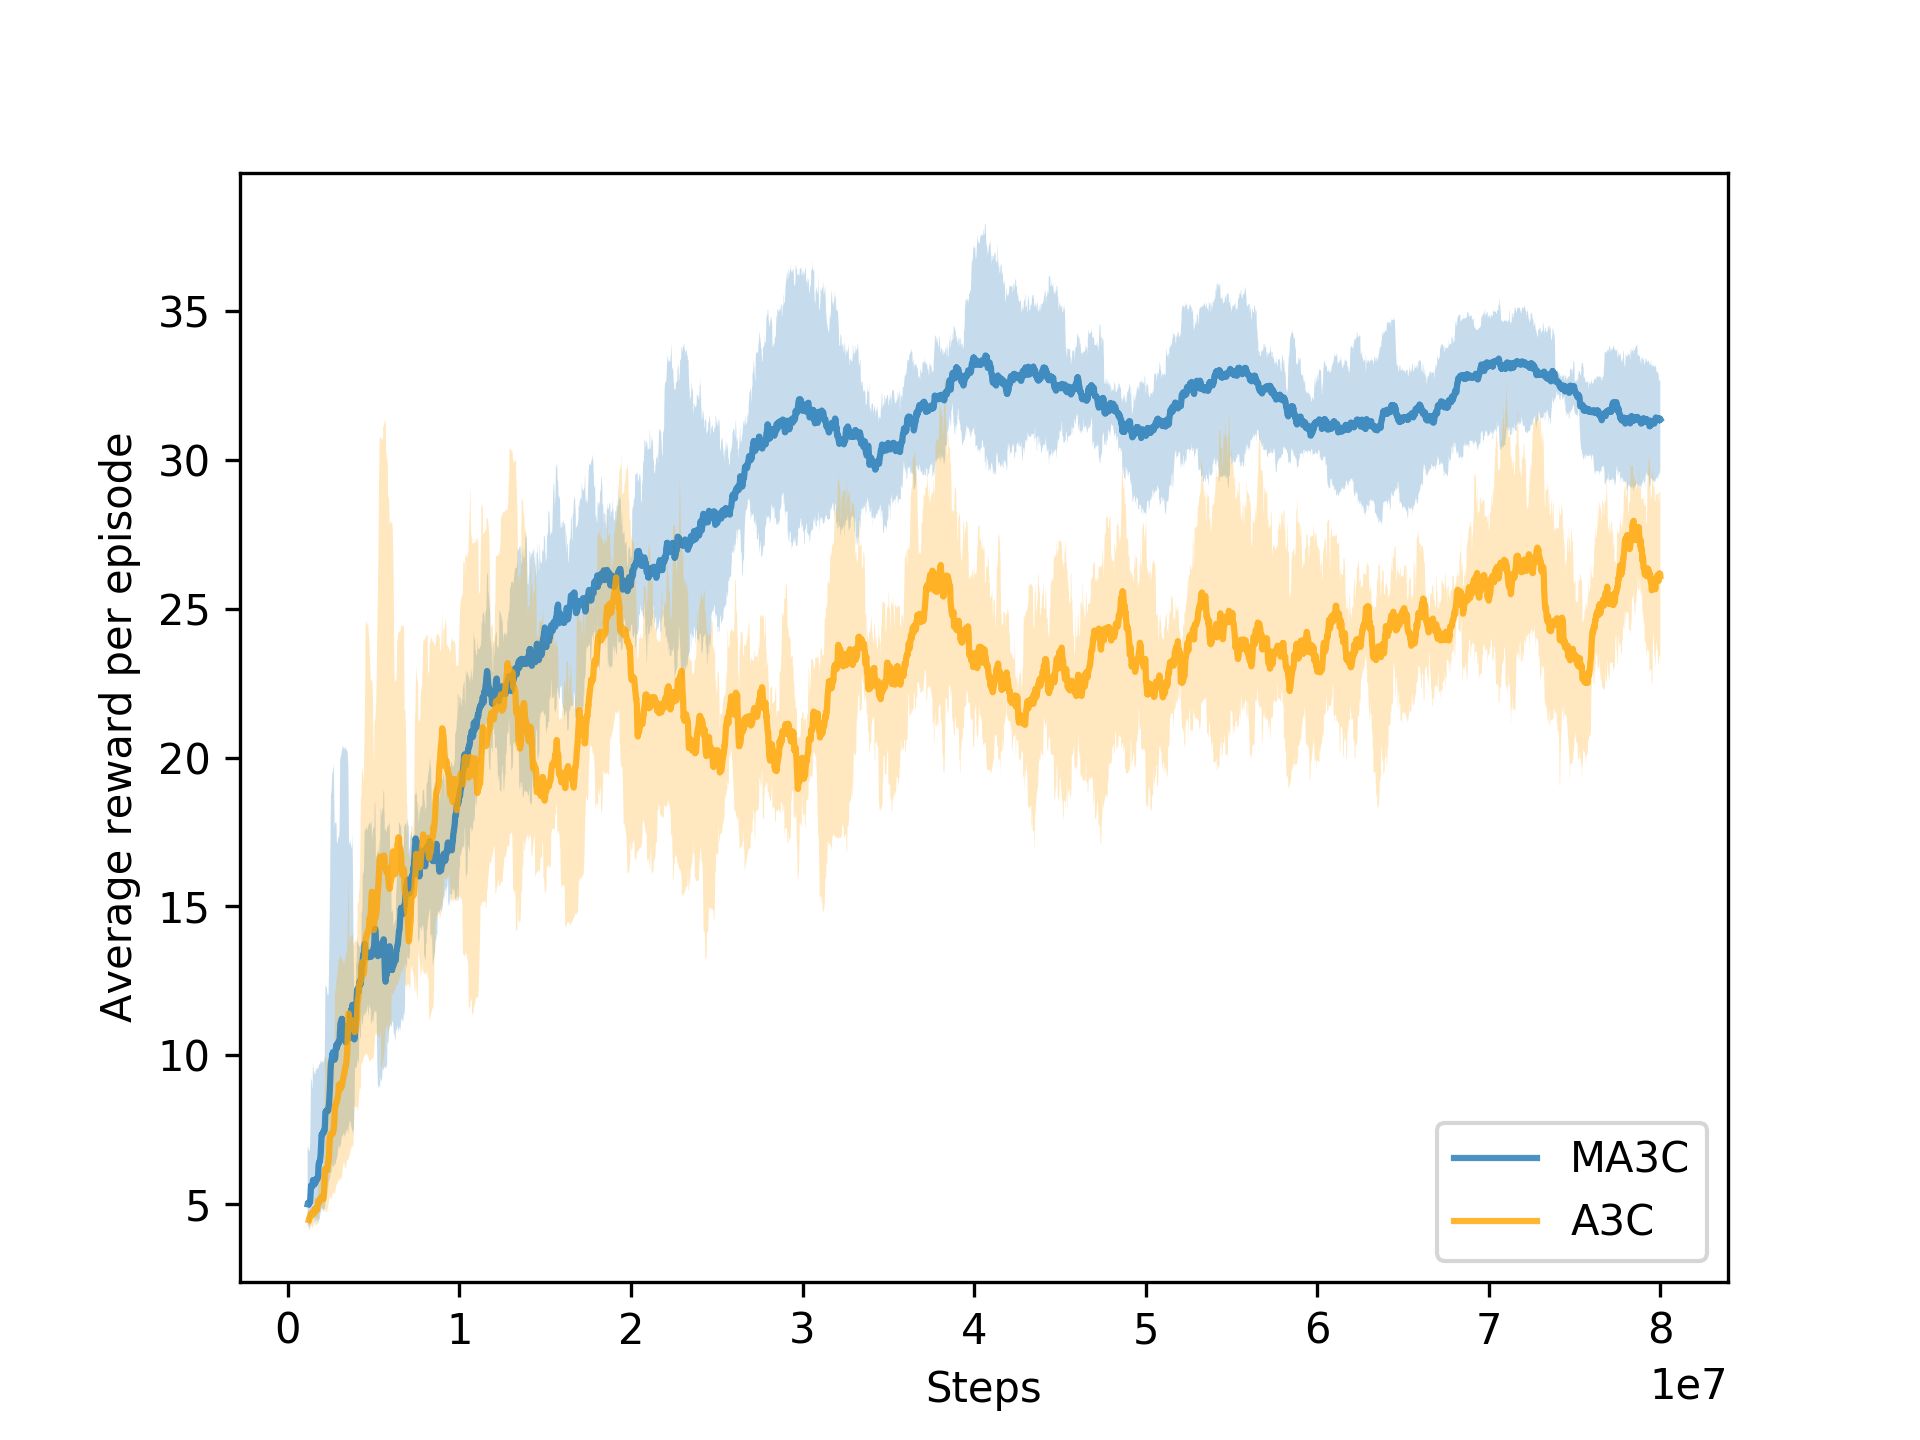
\includegraphics[width=250]{img/Montezuma_performance.png}
\end{center}
\caption[Montezuma's Revenge performance]
{Average score over $5$ runs of \ac{A3C} and \ac{MA3C} algorithms in Simple States environment (80M steps/actions).
The graphics have been smoothed by a moving average with a $20$ steps window.
The shadow represents maximum and minimum values of those $5$ smoothed runs.}
\label{fig:Montezuma_performance}
\end{figure}

As explained in \ffref{subsec:MontezumasRevenge}, the algorithm is learning the different options of the problem (which are
being executed one after the other).
After doing an 80 million steps training, it was able to reach the third checkpoint (Lstairs) in many runs, while reaching
the key in just a few of them.
So it successfully learned the policies of options $o_0$, $o_1$ and $o_2$, and it was trying to learn $o_3$.
This is not fully true because the reward of completing $o_3$ is 110 while the others rewards are just 10, but we can
affirm that with this training process we obtain policies which reach Lstairs with high probability.

As in the other experiments, there might be a different combination of hyperparameters which performs better than in this one,
but they are good enough to show the differences between both algorithms.

% TODO F VER QUE TODAS LAS GRAFICAS SE QUEDEN BIEN

As can be seen in \ffref{fig:Montezuma_performance}, the learning process of \ac{MA3C} is faster than \ac{A3C}.
Even in complex environments as this one is, the main knowledge can be resumed in the first layers and changing the
subtree is useful to model different subgoals/options.
The \ac{MA3C} curve is also less noisy than \ac{A3C}, which means that this algorithm is less susceptible to
behaviour changes during the learning process.

%%% Local Variables: 
%%% mode: latex
%%% TeX-master: "../report"
%%% End: 
\cleardoublepage
\chapter{Conclusions and Future Work}
\section{Conclusions}
First we learned the basics of reinforcement learning, specifically how to model a problem as a \acl{MDP} and how different
algorithms that solve this kind of problems work: Q-learning and \acl{A3C}.
Later, we did a brief introduction to \aclp{ANN}, emphasizing on the architecture of the network and how to improve
the learning process through transfer learning techniques.
We also resumed the state of the art of deep reinforcement learning algorithms to finally propose a variation of those
which take advantage of transfer learning methods.

We developed two simple games and modified one of the most famous Atari games (\acl{MR}) to help us understanding the
strengths of our new algorithm.
We model these games by splitting it into smaller tasks and arranging them in a sequence.
We realized that \ac{MA3C} successfully reused the acquired knowledge of previous tasks in new ones, improving exploration,
learning speed and learning stability.

Thanks of being a really general approach it should be easy to replicate in other games or problems, just by identifying
how to split them.

\section{Future work}

We have managed subgraph changes of \ac{MA3C} in a simple manner, but there are more intelligent ways of doing it.
We could have any kind of \ac{AI} algorithm to select the subgraph which is activated, it would be interesting to analyse
the combination of different algorithms with \ac{MA3C}.
For example, MLSH (\cite{frans2017meta}) is a very similar algorithm which automatically selects the active subgraph.

We made transfer learning through an unsupervised learning approach, but an attractive research would be to transfer the
knowledge in a supervised manner.
A way of doing it is to have just two subgraphs and using one to enhance exploration when the first one converges.
There will be a \ac{MA3C} network whose first subgraph trains in a problem until convergence and then the second subgraph
starts training with all the previous knowledge.
Then if this new subgraph finds another better policy we could use the outputs of this policy to train the first network
in a supervised manner, i.e. by giving input-output pairs to the first subgraph.

One of the main weaknesses of \ac{A3C} is the exploration, and we tried to improve it with \ac{MA3C}, which enhances the
exploration implicitly by promoting randomness.
We realized that there might be a way of modifying the return equation (\ffref{eq:return}) ir order to explicitly add
rewards for exploring new states.

%%% Local Variables: 
%%% mode: latex
%%% TeX-master: "../report"
%%% End: 

\cleardoublepage
\thispagestyle{empty}
\printbibliography
\addcontentsline{toc}{chapter}{Bibliography}

%\appendix
%\chapter{Figures enhanced. Learning revisited.}
Since the presentation of this work on 25 July, 2016, it has been
edited: most figures have been enhanced readability-wise, but its content is
otherwise unchanged. In addition, the learning results have been improved by
using a somewhat different methodology.

The Sarsa agent that employs the options described in \ffref{sec:options}, the
results of which are shown in \ffref{fig:with_options}, has been improved. The
cause of its lack of success was indeed having too negative a reward in the
direction we intended to nudge it, but that was not caused by inadequate
options. Instead, the reason was that the discount rate was too low.

The options skipped no frames ($frame\_skip=1$), as opposed to $frame\_skip=4$
for the non-option version. Thus, the frequency of negative reinforcement by the
shaping function increased, and caused the observed effect. To correct for that,
we set the discount rate $\gamma=0.9995$, which is larger than $\sqrt[4]{0.995}$
but close.

The results can be seen in \ffref{fig:with_options_9995}. Observe that the
rewards towards the end are much lower than in the option-less agent in
\ffref{fig:without_options}. Also, the non-annealed agent has trouble finding
the reward consistently in the beginning, but does find it within the first few
thousand episodes.

\drawtraining{with_options_9995}{Same as \ffref{fig:with_options}, but with
  $\gamma=0.9995$. Annealed, blue uses $\varepsilon=\textsc{Max}(0.1, 0.7 -
  10^{-4} \cdot n_e)$. Red uses $\varepsilon=0.1$.}

Counter-intuitively, the agent was still learning more
slowly with options than without. This seemed be in great part because of
the relatively infrequent updates: the option-based agent updated the $Q$ table
once per option, which usually last more than 10 frames, while the agent without
options updated once every 4 frames.

Accordingly, we changed the algorithm to update the action-value of an option
every frame. Let the agent initiate an option $o_t$ at time $t$, which
finishes at time $t+k$. Because of how we defined our options
(\ffref{sec:options}), we know that for all $t'$ such that $t \leq t' < t+k$,
$s_{t'} \in \mathcal{I}_{o_t}$. That is, an option can be started in any state
that is reached when executing it. Thus, we can use the update in
\ffref{eq:options-q-update} for all intermediate states $t'$:
\begin{equation}
  \begin{array}{c}
  Q(s_t, o_t) \gets (1-\alpha)Q(s_t, o_t) + \alpha \left[r_{t:t+k} + \gamma^k
Q(s_{t+k}, o_{t+k}) \right] \\
Q(s_{t+1}, o_t) \gets (1-\alpha)Q(s_{t+1}, o_t) + \alpha \left[r_{t+1:t+k} +
\gamma^{k-1} Q(s_{t+k}, o_{t+k}) \right] \\
\dots \\
Q(s_{t+k-1}, o_t) \gets (1-\alpha)Q(s_{t+k-1}, o_t) + \alpha \left[r_{t+k-1} +
\gamma Q(s_{t+k}, o_{t+k}) \right]
 \end{array}
\end{equation}

This algorithm is very similar to the forward view $k$-step return
Sarsa($\lambda$) \citep[Sections~7.1,~7.2,~7.5]{sutton1998introduction}. In this
case, $k$ is not necessarily equal every time an option is executed.

The results of using this improvement can be seen in
\ffref{fig:with_options_each_frame}. The blue agent, the best performing,
achieves 0.5 more average reward per episode than the previously best performing
option-less agent, in 1/25 the number of training episodes. It is worth noting
that the option-less agent uses $\varepsilon=0.1$ in the end, compared to
$\varepsilon=0.01$ from this agent, and that performing the wrong option has
more far-reaching consequences than choosing the wrong action.

\drawtraining{with_options_each_frame}{Reward per episode, averaged every 1000
episodes, as the training progresses. Options are used. Red uses
$\varepsilon=\textsc{Max}(0.01, 0.2 - 10^{-3} \cdot n_e)$, blue uses
$\varepsilon=\textsc{Max}(0.01, 0.2 - 10^{-4} \cdot n_e)$, amber uses
$\varepsilon=0.1$ and green uses $\varepsilon=0.05$. All use $\gamma=0.9995$.
Darker lines, with higher value, do not include the shaping reward $F(\cdot)$;
lighter lines show the reward as the agent experiences it. $y$ axis is reward,
$x$ axis is thousands of episodes.}

Seeing the success of this modification, we applied it back to the
option-less agent. We framed each action with $frame\_skip=4$ as an option that
takes the 1-frame action for 4 frames, and applied the same algorithm. The
results can be seen in figure \ffref{fig:without_options_each_frame}. In general
we observe that how fast the agent learns depends on the annealing rate, but the
final performance depends only on the final $\varepsilon$.

\drawtraining{without_options_each_frame}{Reward per episode, averaged every 1000
episodes, as the training progresses. No options are used. Red uses
$\varepsilon=\textsc{Max}(0.01, 0.7 - 10^{-4} \cdot n_e)$, blue uses
$\varepsilon=\textsc{Max}(0.01, 0.7 - 5 \cdot 10^{-5} \cdot n_e)$, amber uses
$\varepsilon=\textsc{Max}(0.1, 0.7 - 10^{-4} \cdot n_e)$ and green uses
$\varepsilon=0.1$. All use $\gamma=0.9995$. Darker lines, with higher value, do
not include the shaping reward $F(\cdot)$; lighter lines show the reward as the
agent experiences it. $y$ axis is reward, $x$ axis is thousands of episodes.}

%%% Local Variables:
%%% mode: latex
%%% TeX-master: "../report"
%%% End:

\end{document}
